%%
%% This file can be distributed and/or modified under the
%% conditions of the LaTeX Project Public License, either version 1.3
%% of this license or (at your option) any later version.
%% The latest version of this license is in
%%   http://www.latex-project.org/lppl.txt
%% and version 1.3 or later is part of all distributions of LaTeX
%% version 2003/12/01 or later.
%% 
%% This work has the LPPL maintenance status "maintained".
%% 
%% The Current Maintainer of this work is Lars Madsen (daleif@imf.au.dk).
%%
%% $LastChangedDate: 2010-05-10 11:02:27 +0200 (Mon, 10 May 2010) $
%% $LastChangedRevision: 784 $
%%
%$
\documentclass[letterpaper,11pt,openany]{memoir}
\def\MyFileVersion{Version 1.7b, 2010/05/10}
\setlrmarginsandblock{2.5cm}{*}{1} 
\setulmarginsandblock{2.5cm}{2.5cm}{*}
\setmarginnotes{2.5mm}{2cm}{1em}
\checkandfixthelayout
\usepackage[latin1]{inputenc}
\usepackage[english]{babel}
\usepackage[T1]{fontenc}
\usepackage{
  calc,
  graphicx,
  url,
  fancyvrb,
  multicol,
  kvsetkeys
}
\usepackage[svgnames,dvipsnames]{xcolor}
\definecolor{felinesrcbgcolor}{rgb}{1,1,0.85}
\definecolor{felinesrcbgcolor}{rgb}{0.94,0.97,1}
\definecolor{felineframe}{rgb}{0.79,0.88,1}
\definecolor{myorange}{rgb}{1,0.375,0}
\definecolor{mycolor}{rgb}{0,0.4,0.2}

\usepackage[draft]{fixme}
\usepackage{fourier}
\usepackage[scaled]{luximono}
\newcommand\starbreak{\fancybreak{\decosix\quad\decosix\quad\decosix}}

%\newcommand\starbreak{\fancybreak{$*\quad*\quad*$}}

\usepackage[scaled]{berasans}
\usepackage{multirow}

%\renewcommand*{\cftchaptername}{\textcolor{black}{\chaptername}~}
%\renewcommand*{\cftchapterfont}{\textcolor{black}{}}

\chapterstyle{ell}
\renewcommand\tocheadstart{}
\renewcommand\printtoctitle[1]{}

\raggedbottom
\fvset{frame=lines,
  framesep=-0.05in,
  framerule=0pt,
  fontsize=\footnotesize,
  rulecolor=\color{myorange},
%  formatcom=\color{DarkGreen},
  formatcom=\color{mycolor},
}
\newoutputstream{StyleList}
 \newoutputstream{OutputStyle}%
 \openoutputfile{\jobname.styles}{StyleList}
\def\OutputStylePostfix{-style}
\def\CurrentChapterStyle{}
\makeatletter
\kv@set@family@handler{MCS}{%
  \xdef\CurrentChapterStyle{#1}%
}
\define@key{MCS}{pages}{%\typeout{xxx: #1}
  \global\@namedef{MCS@pages@\CurrentChapterStyle}{#1}%
}
\newif\ifSCS@full
\newcounter{MCS}
\newenvironment{@showchapterstyle}[1]{%
  \kvsetkeys{MCS}{#1}%
  \ifSCS@full%
    \edef\hest{\CurrentChapterStyle\OutputStylePostfix\space page \@nameuse{MCS@pages@\CurrentChapterStyle}}
    \addtostream{StyleList}{\hest}%
  \else%
    \addtostream{StyleList}{\CurrentChapterStyle\OutputStylePostfix}%
  \fi%
  \openoutputfile{\CurrentChapterStyle\OutputStylePostfix.tex}{OutputStyle}%
  \ifSCS@full%
    \addtostream{OutputStyle}{%
      \protect\let\protect\STARTCODE\relax^^J%
      \protect\let\protect\STOPCODE\relax^^J%
      \protect\STARTCODE%
    }%
  \else%
    \addtostream{OutputStyle}{%
      \protect\documentclass{memoir}^^J%
      \protect\let\protect\STARTCODE\relax^^J%
      \protect\let\protect\STOPCODE\relax^^J%
      \protect\STARTCODE%
    }%
  \fi%
  \writeverbatim{OutputStyle}%
}{%
  \endwriteverbatim\relax%
  \ifSCS@full%
    \addtostream{OutputStyle}{%
      \protect\STOPCODE%
    }
  \else% 
    \addtostream{OutputStyle}{%
      \protect\chapterstyle{\CurrentChapterStyle}^^J%
      \protect\STOPCODE^^J%
      \protect\setlength\afterchapskip{\onelineskip}^^J%
      \protect\setlength\beforechapskip{\onelineskip}^^J%
      \protect\usepackage{lipsum}^^J%
      \protect\begin{document}^^J%
      \protect\input{chapterexample.tex}^^J%
      \protect\end{document}%
    }%
  \fi%
  \closeoutputstream{OutputStyle}%
  \edef\FancyVerbStartString{\string\STARTCODE}%
  \edef\FancyVerbStopString{\string\STOPCODE}%
  \vskip\z@\@plus\bottomsectionskip
  \penalty\z@
  \vskip\z@\@plus -\bottomsectionskip
  \phantomsection
  \addcontentsline{toc}{section}{\CurrentChapterStyle}
  \VerbatimInput[label={\small Source for the \textsf{\CurrentChapterStyle} style}]{\CurrentChapterStyle-style.tex}%%
  \par\noindent%
  \IfFileExists{\CurrentChapterStyle\OutputStylePostfix.pdf}{%
    \fboxsep=4pt%
    \begin{adjustwidth}{-\fboxsep-\fboxrule}{-\fboxsep-\fboxrule}%
%      \begin{framed}%
        \@ifundefined{MCS@pages@\CurrentChapterStyle}{%
          \fcolorbox{felineframe}{felinesrcbgcolor}{\includegraphics[width=\textwidth]{\CurrentChapterStyle\OutputStylePostfix}}%
        }{%
          \edef\nisse{\@nameuse{MCS@pages@\CurrentChapterStyle}}
          \@for\ITEM:=\nisse\do{
            \ifpdf%
              \fcolorbox{felineframe}{felinesrcbgcolor}{\includegraphics%
              [width=\textwidth,page=\ITEM]{\CurrentChapterStyle\OutputStylePostfix}}%
            \else%
              \fcolorbox{felineframe}{felinesrcbgcolor}{\includegraphics%
              [width=\textwidth]{\CurrentChapterStyle\OutputStylePostfix-\ITEM}}%
            \fi%
            \bigskip%
            \fancybreak{$***$}%
            \bigskip
          }%
        }%
%      \end{framed}%
    \end{adjustwidth}
  }{\fbox{File \CurrentChapterStyle-style.* does not exist}}
  \vskip1em plus 1em minus -.5em\noindent%
}
% the two actual environments, the stared one will let you add entire
% documents, while the unstared one will only display sniplets
\newenvironment{showchapterstyle}[1]{%
\SCS@fullfalse\@showchapterstyle{#1}}{\end@showchapterstyle}
\newenvironment{showchapterstyle*}[1]{%
\SCS@fulltrue\@showchapterstyle{#1}}{\end@showchapterstyle\SCS@fullfalse}
\newcommand\@Arg[1]{\textnormal{$\langle$\textit{#1}$\rangle$}}
\newcommand\@Args[1]{\texttt{\{\textnormal{$\langle$\textit{#1}$\rangle$}\}}}
\newcommand\Arg{\@ifstar{\@Args}{\@Arg}}
\renewcommand\cs[1]{\texttt{\textbackslash #1}}
%%%%%%%%%%%%%%%%%%%%%%%%%%%%%%%%%%%%%%%%%%%%%%%%%%%%%%%%%%%%%%%%%%%%%%%%%%%%%%%%%%%%
% for continuous numbering
\counterwithout*{figure}{chapter}
\counterwithout*{table}{chapter}
\counterwithout*{equation}{chapter}
\renewcommand{\thefigure}{\@arabic\c@figure}
\renewcommand{\thetable}{\@arabic\c@table}
\renewcommand{\theequation}{\@arabic\c@equation}
\setcounter{secnumdepth}{3}
\g@addto@macro{\appendixpage}{%
  \addtocontents{toc}{%
    \protect\renewcommand{\protect\cftchapterfont}{}%
  }%
}
\newcommand{\urlc}[1]{\textcolor{WildStrawberry}{\url{#1}}}
%%%%%%%%%%%%%%%%%%%%%%%%%%%%%%%%%%%%%%%%%%%%%%%%%%%%%%%%%%%%%%%%%%%%%%%%%%%%%%%%%%%%
\makeatother
\newenvironment{syntax}{%
  \vskip.5\onelineskip%
  \begin{adjustwidth}{0pt}{0pt}
    \parindent=0pt%
    \obeylines%
    \let\\=\relax%
  }{%
  \end{adjustwidth}%
  \vskip.5\onelineskip%
}
\newenvironment{syntax*}{%
  \vskip.5\onelineskip%
  \begin{adjustwidth}{0pt}{0pt}
    \parindent=0pt%
  }{%
  \end{adjustwidth}%
  \vskip.5\onelineskip%
}

\newtheorem{remark}{Remark}

\AtEndDocument{\closeoutputstream{StyleList}}
\pagestyle{plain}

\ifpdf
\usepackage{hyperref}
\hypersetup{
%  colorlinks,
%  citecolor=PineGreen,
%  linkcolor=black,
%  urlcolor=WildStrawberry,
  urlbordercolor=white,
  citebordercolor=PineGreen,
}
\fi
%%%%%%%%%%%%%%%%%%%%%%%%%%%%%%%%%%%%%%%%%%%%%%%%%%%%%%%%%%%%%%%%%%%%%%%%%%%%%%%%%%%%%%
\newcommand{\SIM}{MacSim\xspace}
\newcommand{\bin}{\textcolor{MidnightBlue}{macsim}\xspace}
\newcommand{\ignore}[1]{}
\newcommand{\cpu}{x86\xspace}
\newcommand{\gpu}{GPU\xspace}

\usepackage{
  xspace,
  graphicx,
  color,
  xcolor,
  listings,
  paralist,
  cite,
  todonotes,
}
%  palatino,


%\lhead{}
%\chead{\small In the proceedings of the 18th IEEE International Symposium on High Performance Computer Architecture (HPCA), February 2012}
%\rhead{}
%\lfoot{}
%\cfoot{\thepage}
%\rfoot{}
%\renewcommand{\headrulewidth}{0pt}
%\renewcommand{\footrulewidth}{0.4pt}
%\pagestyle{myheadings}
%\pagenumbering{arabic}
%\setlength{\headsep}{0.35in}
%\setlength{\voffset}{-0.35in}



\usepackage[labelsep=period, font={singlespacing}, labelfont={bf}, textfont={rm}, skip=5pt]{caption}


%\usepackage{graphicx}
%\usepackage{color}
%\usepackage{xcolor}
%\usepackage{xspace}
%\usepackage{listings}
\lstset{columns=fullflexible,basicstyle=\footnotesize\ttfamily}
%\usepackage{paralist}
%\usepackage{cite}

%%%%%%%%%%%%%%%%%%%%%%%%%%%%%%%%%%%%%%%%%%%%%%%%%%%%%%%%%%%%%%%%%%%%%%%%%%%%%%%%%%%%%%

\begin{document}

\thispagestyle{empty}
\vspace*{\fill}
\begin{center}
\HUGE\textsf{MacSim: A CPU-GPU Heterogeneous Simulation Framework}\par
\end{center}

\begin{center}
\Huge\textsf{User Guide}\par
\end{center}

\vspace*{\fill}

\begin{center}
\Large\textsf{Hyesoon Kim}\par
\Large\textsf{Jaekyu Lee}\par
\Large\textsf{Nagesh B. Lakshminarayana}\par
\Large\textsf{Jaewoong Sim}\par
\Large\textsf{Jieun Lim}\par
\Large\textsf{Tri Pho}\par
\end{center}
\vspace*{\fill}
\begin{center}
\textrm{HPArch research group}\\
\textrm{(\url{http://comparch.gatech.edu/hparch/index.html})} \\
\textsf{Georgia Institute of Technology} \\[0.2\baselineskip]
\setlength{\droptitle}{0pt}%
\end{center}
\clearpage


%\starbreak
%The sample text used is
%\VerbatimInput[
%label={chapterexample.tex},
%fontsize=\small
%]{chapterexample.tex}

%\begin{Verbatim}
%\let\STARTCODE\relax 
%\let\STOPCODE\relax 
%\STARTCODE
%...
%\STOPCODE  
%\end{Verbatim}


%\begingroup
%\renewcommand\descriptionlabel[1]{\hspace\labelsep\cs{#1}}
%\begin{description}\firmlist
%\item[beforechapskip] length, self explanatory,usually set using
%  \verb+\chapterheadstart+, default 50pt
%\item[midchapskip] length, distance between the chapter name / number and the
%title, usually set using \verb+\afterchapternum+, default 20pt
%\item[afterchapskip] length, distance between the chapter title and
%  the following text, usually set using \verb+\afterchaptertitle+,
%  default 40pt
%\item[chapnamefont] the font setting used for \emph{Chapter} or
%  similar, default \verb+\normalfont\huge\bfseries+
%\item[chapnumfont] same for the chapter number, default
%  \verb+\normalfont\huge\bfseries+
%\item[chaptitlefont] same for the chapter title, default
%  \verb+\normalfont\Huge\bfseries+ 
%\end{description}
%\endgroup



\chapter*{\contentsname}
\tableofcontents*


%setlength\columnsep{8mm}
%begin{multicols}{1}
% \tableofcontents*
%end{multicols}

\newpage

\ignore {\listoftodos}




%%%%%%%%%%%%%%%%%%%%%%%%%%%%%%%%%%%%%%%%%%%%%%%%%%%%%%%%%%%%%%%%%%%%%%%%
\chapter{Introduction}
%%%%%%%%%%%%%%%%%%%%%%%%%%%%%%%%%%%%%%%%%%%%%%%%%%%%%%%%%%%%%%%%%%%%%%%%


\SIM is a heterogeneous architecture simulator, which is trace-driven
and cycle-level. It thoroughly models architectural behaviors,
including detailed pipeline stages, multi-threading, and memory
systems. Currently, \SIM support x86 and NVIDIA PTX instruction set
architectures (ISA). \SIM is capable of simulating a variety of
architecreus, such as Intel's Sandy Bridge~\cite{sandybridge} and
NVIDIA's Fermi~\cite{fermi}.  It can simulate homogeneous ISA
multicore simulations as well as heterogeneous ISA multicore
simulations.

MacSim is a microarchitecture simulator that simulates detailed
pipeline (in-order and out-of-order) and a memory system including
caches, NoC, and memory controllers. It supports, asymmetric multicore
configurations (small cores + medium cores + big cores) and SMT or MT
architectures as well.

Currently interconnection network model (based on IRIS) and power
model (based on McPat~\cite{mcpat}) are connected. ARM ISA support is
on-progress. MacSim is also one of the components of SST~\cite{sst} so
multiple MacSim simulators can run concurrently.





%%%%%%%%%%%%%%%%%%%%%%%%%%%%%%%%%%%%%%%%%%%%%%%%%%%%%%%%%%%%%%%%%%%%%%%%
\section*{Macsim version information}
%%%%%%%%%%%%%%%%%%%%%%%%%%%%%%%%%%%%%%%%%%%%%%%%%%%%%%%%%%%%%%%%%%%%%%%%


\begingroup
\renewcommand\descriptionlabel[1]{\textit{\hspace\labelsep{#1}}}
%\renewcommand\descriptionlabel[1]{\hspace\labelsep\cs{#1}}
\begin{description}\firmlist
\item[1.0 - February xx, 2012] Initial release

  \Verb+macsim-top/tags/macsim_1.0+ 
\end{description}
\endgroup
















% LocalWords:  Macsim MacSim NVIDIA PTX multicore RISC uops microarchitecture
% LocalWords:  NoC SMT McPat



%%%%%%%%%%%%%%%%%%%%%%%%%%%%%%%%%%%%%%%%%%%%%%%%%%%%%%%%%%%%%%%%%%%%%%%%
\chapter{Getting Started}
%%%%%%%%%%%%%%%%%%%%%%%%%%%%%%%%%%%%%%%%%%%%%%%%%%%%%%%%%%%%%%%%%%%%%%%%


This chapter provides instructions for building, installing, and running \SIM.


%%%%%%%%%%%%%%%%%%%%%%%%%%%%%%%%%%%%%%%%%%%%%%%%%%%%%%%%%%%%%%%%%%%%%%%%
\section{Documentation and Other Support}
%%%%%%%%%%%%%%%%%%%%%%%%%%%%%%%%%%%%%%%%%%%%%%%%%%%%%%%%%%%%%%%%%%%%%%%%

\SIM is hosted on Google Code at the following URL:
\urlc{http://code.google.com/p/macsim}. The project page for \SIM on
Google Code provides stable version of \SIM, detailed documentation,
issue/bug tracking, sample traces and so on. Users can use the project
page for filing issues and for contacting the maintainers of \SIM.


%%%%%%%%%%%%%%%%%%%%%%%%%%%%%%%%%%%%%%%%%%%%%%%%%%%%%%%%%%%%%%%%%%%%%%%%
\section{Building \SIM}
\label{sec:installation}
%%%%%%%%%%%%%%%%%%%%%%%%%%%%%%%%%%%%%%%%%%%%%%%%%%%%%%%%%%%%%%%%%%%%%%%%


%%%%%%%%%%%%%%%%%%%%%%%%%%%%%%%%%%%%%%%%%%%%%%%%%%%%%%%%%%%%%%%%%%%%%%%%
\subsection{Obtaining Source}
%%%%%%%%%%%%%%%%%%%%%%%%%%%%%%%%%%%%%%%%%%%%%%%%%%%%%%%%%%%%%%%%%%%%%%%%

\SIM source code is maintained using subversion. Users can obtain a copy of the
source code using this command:

\begin{Verbatim}
svn co https://svn.research.cc.gatech.edu/macsim/trunk macsim-readonly --username readonly
\end{Verbatim}

\noindent
Note that currently password is not set for readonly account, so
`enter' when you prompt password. Due to the technical issue, we do
not allow anonymous checkout now. As soon as the issue has been
resolved, we will update this documentation.

Users will have read-only permission by default and users interested
in contributing to \SIM must contact
\href{mailto:macsim-dev@googlegroups.com}{macsim-dev@googlegroups.com}.



%%%%%%%%%%%%%%%%%%%%%%%%%%%%%%%%%%%%%%%%%%%%%%%%%%%%%%%%%%%%%%%%%%%%%%%%
\subsection{Requirements}
%%%%%%%%%%%%%%%%%%%%%%%%%%%%%%%%%%%%%%%%%%%%%%%%%%%%%%%%%%%%%%%%%%%%%%%%

To build \SIM the following are required:

\begingroup
\renewcommand\descriptionlabel[1]{\textit{\hspace\labelsep{#1}}}
%\renewcommand\descriptionlabel[1]{\hspace\labelsep\cs{#1}}
\begin{description}\firmlist
  \item[Operating System] At present only Linux distributions are supported. \SIM has been tested on:
   \Verb+Ubuntu+, \Verb+Redhat (TODO)+
  \item[Compiler] Any compiler that supports the C++0x (or C++11)
    standard. \SIM has been verified to work with: \Verb+gcc 4.4 or higher+, \Verb+icc (will work on)+
  \item[Autotools] - Autotools (automake, autoconf,
    ...) version 2.65 or higher is required. Autotools can be installed using the commands:
\begin{Verbatim}
Ubuntu: apt-get install autotools-dev automake autoconf
Redhat: todo
\end{Verbatim}
  \item[Libraries] - The zlib library is required and it can be installed using the command:
\begin{Verbatim}
Ubuntu: apt-get install zlib1g-dev
\end{Verbatim}
\end{description}
\endgroup




\ignore{
\subsection{Directory Structure}

This section explains the directory structure of \SIM simulator.

\smallskip
\begin{lstlisting}
macsim/
  tag/ branch/ trunk/
\end{lstlisting}
\smallskip

\textit{Tag} directory has tagged version of \SIM
simulators. \textit{Branch} directory is for diverged \SIM, which is
currently empty. \textit{Trunk} directory is current working directory
for \SIM.

Following is more detailed information about \textit{Trunk} directory.

\smallskip
\begin{lstlisting}
trunk/
  bin/ def/ doc/ params/ scripts/ src/ tools/
\end{lstlisting}
\smallskip

\textit{Bin} directory contains the \SIM binary after the building
process. \textit{def} directory has knob (Section~\ref{sec:knob}) and
statistics (Section~\ref{sec:stat}) definitions. \textit{doc} has the
documentation. \textit{scripts} includes several scripts files that
are using during the building process. \textit{src} contains all
source files. \textit{tools} has several useful tools.
\ignore{ (Section~\ref{sec:tool}) }
}

\ignore
{
%%%%%%%%%%%%%%%%%%%%%%%%%%%%%%%%%%%%%%%%%%%%%%%%%%%%%%%%%%%%%%%%%%%%%%%%
\subsection{Source organization}
%%%%%%%%%%%%%%%%%%%%%%%%%%%%%%%%%%%%%%%%%%%%%%%%%%%%%%%%%%%%%%%%%%%%%%%%

\TODO{check this, i'm not sure what is included in the copy that be available
  publically} 

The top-level source directory of \SIM contains several source, script and tool
directories, README and INSTALL files and files required for building \SIM
using autotools. Below is a brief description of the contents of the top-level
source directory of \SIM.


\begin{description}\firmlist

\item [bin] Build output directory.

\item [def] Contains definitions of parameters (see Sections~\ref{sec:run}
    and~\ref{sec:knob}) and events for statistics (see Section~\ref{sec:stat}).

\item [doc] Contains \SIM documentation.

\item [params] Contains sample parameter (see Sections~\ref{sec:run}
    and~\ref{sec:knob}) configuration files.

\item [scripts] Contains scripts used in build of \SIM.

\item [src] Contains \SIM source files (.cc and .h files).

\item [tools] Contains x86 trace generator and trace reader.

\item [README, INSTALL] README and INSTALL files containing proceduce to build
and run \SIM and patch \SIM to make it usable as a SST component (see
    Section~\ref{sec:sst}).

\item [autogen.sh] Script file to generate makefile to build \SIM.

\item [configure.in aclocal.m4 Makefile.am Makefile.in] Files required by
autotools to generate makefile to build \SIM.


\end{description}
}

\ignore
{
  The top-level source directory of \SIM contains several directories including
  \Verb+bin+, \Verb+def+, \Verb+doc+, \Verb+params+, \Verb+scripts+, \Verb+src+ and
  \Verb+tools+ and the \Verb+README+ and \Verb+INSTALL+ files and the files
  required for building \SIM using autotools.
}


%%%%%%%%%%%%%%%%%%%%%%%%%%%%%%%%%%%%%%%%%%%%%%%%%%%%%%%%%%%%%%%%%%%%%%%%
\subsection{Build}
%%%%%%%%%%%%%%%%%%%%%%%%%%%%%%%%%%%%%%%%%%%%%%%%%%%%%%%%%%%%%%%%%%%%%%%%

The GNU Autotools (aclocal, automake, autoconf, ...) are used to build \SIM.
After checking out a copy of the \SIM source code, the following commands have
to be executed (These instructions are also available in \Verb+INSTALL+ file
    included in the \SIM source).


\begin{Verbatim}
aclocal 
automake 
--add-missing 
autoconf 
./configure 
make
\end{Verbatim}

\noindent
Users can enter all the above commands in one go as shown below:

\begin{Verbatim}
aclocal && automake --add-missing && autoconf && ./configure && make
\end{Verbatim}

\noindent Alternatively, users can just run the autogen.sh script file included
in the \SIM source and then run the \Verb+make+ to build \SIM.

\begin{Verbatim}
./autogen.sh
make
\end{Verbatim}

\noindent
On a successful build, the binary \bin will be generated in the \Verb+trunk/bin/+
directory.




%%%%%%%%%%%%%%%%%%%%%%%%%%%%%%%%%%%%%%%%%%%%%%%%%%%%%%%%%%%%%%%%%%%%%%%%
\subsection{Build Types}
%%%%%%%%%%%%%%%%%%%%%%%%%%%%%%%%%%%%%%%%%%%%%%%%%%%%%%%%%%%%%%%%%%%%%%%%

Three types of build, each of which uses different compiler flags are
supported. The build types are:

\begin{itemize}
  \item opt : default, optimized version (-O3 flag)
  \item dbg : debug version (-g3 flag)
  \item gpf : gprof version (-pg flag)
\end{itemize}

\noindent
The build type can be specified as an argument to the \textit{make} command.

\begin{Verbatim}
To build the optimized version of the binary
make [opt] 

To build the debug version of the binary
make dbg

To build the gprof version of the binary
make gpf
\end{Verbatim}





%%%%%%%%%%%%%%%%%%%%%%%%%%%%%%%%%%%%%%%%%%%%%%%%%%%%%%%%%%%%%%%%%%%%%%%%
\section{Running \SIM}
\label{sec:run}
%%%%%%%%%%%%%%%%%%%%%%%%%%%%%%%%%%%%%%%%%%%%%%%%%%%%%%%%%%%%%%%%%%%%%%%%

To run \bin binary, two additional files are required to be present 
the same directory as the binary.

\begin{itemize}
  \item params.in - defines architectural parameter values that will
  overwrite the default parameter values.

  \item trace\_file\_list - specifies the number of traces to run and
  the location of each trace.
\end{itemize}


Several pre-defined architectural parameter configuration files are provided in
\Verb+macsim-top/trunk/params+ directory. Table~\ref{table:param} lists the
pre-defined parameter files. To run \SIM with a particular architectural
configuration, users should copy the corresponding parameter file to \Verb+bin+
directory and rename it as \Verb+params.in+. For example, to use NVIDIA's
Fermi~\cite{fermi} GPU architecture, \Verb+params/params_gtx465+ should be
copied to \Verb+bin+ and renamed as \Verb+params.in+. 



\ignore{
We provide several pre-defined architecture parameters in
\Verb+macsim-top/trunk/params+ directory. Table~\ref{table:param}
shows the list of pre-defined parameter files. If you want to run \SIM
with a certain configuration, you need to copy the corresponding
parameter file to \Verb+bin+ directory and rename it as
\Verb+params.in+. For example, if you want to use NVIDIA's
Fermi~\cite{fermi} GPU architecture, the following command would be
sufficient:

\begin{Verbatim}
cp params/params_gtx465 bin/params.in
\end{Verbatim}
}

\begin{table}
\begin{footnotesize}
\begin{center}
\caption{Parameter Templates}
\label{table:param}
\begin{tabular}{|l|l|l|}
\hline
File Name              & Description & Architecture                         \\ \hline \hline
params\_8800gt         &             & NVIDIA GeForce 8800 GT (G80)         \\
params\_gtx280         &             & NVIDIA GeForce GTX 280 (GT200)       \\
params\_gtx465         &             & NVIDIA GeForce GTX 465 (Fermi)       \\
params\_x86            &             & Intel's Sandy Bridge (CPU part only) \\
params\_hetero\_4c\_4g &             & Intel's Sandy Bridge (CPU + GPU)     \\ \hline
\end{tabular}
\end{center}
\end{footnotesize}
\end{table}


\Verb+trace_file_list+ specifies the list of traces to be simulated. Following is the
content of a sample \Verb+trace_file_list+.

\begin{Verbatim}
2 <-- number of traces
/trace/ptx/cuda2.2/FastWalshTransform/kernel_config.txt <-- trace 1 path
/trace/ptx/cuda2.2/BlackScholes/kernel_config.txt <-- trace 2 path
\end{Verbatim}

\noindent

Above, the first line specifies the number of traces (applications) that will
be simulated and each line thereafter specifies the path to the trace
configuration file in the trace directory of an application. The contents of a
sample trace configuration file are shown below.

\begin{Verbatim}
1 x86
0 0
\end{Verbatim}

\noindent In the first line, the first field indicates the number of threads in
the application (1 in this case) and the second field specifies the type of the
application (x86 in this case). Other lines contain a thread id and the starting 
point of the thread in terms of the instruction count of the main thread
(thread 0).


Several sample trace files are available at
\urlc{http://code.google.com/p/macsim}. Users can generate their own
traces by following instructions in Chapter~\ref{ch:trace}.


%%%%%%%%%%%%%%%%%%%%%%%%%%%%%%%%%%%%%%%%%%%%%%%%%%%%%%%%%%%%%%%%%%%%%%%%
\subsection{Run}
%%%%%%%%%%%%%%%%%%%%%%%%%%%%%%%%%%%%%%%%%%%%%%%%%%%%%%%%%%%%%%%%%%%%%%%%

The \SIM simulator can be run by executing the \bin binary located in the
\Verb+trunk/bin/+ directory.

\begin{Verbatim}
./macsim
\end{Verbatim}



%%%%%%%%%%%%%%%%%%%%%%%%%%%%%%%%%%%%%%%%%%%%%%%%%%%%%%%%%%%%%%%%%%%%%%%%
\section{Output}
%%%%%%%%%%%%%%%%%%%%%%%%%%%%%%%%%%%%%%%%%%%%%%%%%%%%%%%%%%%%%%%%%%%%%%%%

\SIM generates a \Verb+params.out+ file and several files \Verb+.stat.out+
containing statistics at the end of a successful simulation. Users can specify
the output directory for these files by setting the
\Verb+STATISTICS\_OUT\_DIRECTORY+ parameter whose default value is the
directory containing the \bin binary. Simulation parameters are discussed in
detail in Section~\ref{sec:knob}.

\ignore{
several output files once the simulation is completed successfully.
 Here are the list of output files.

\begin{Verbatim}
params.out
statfile1.stat.out
statfile2.stat.out
...
statfilen.stat.out
\end{Verbatim}
}

\noindent \Verb+params.out+ enumerates all parameters with their values used
for the simulation. The \Verb+.stat.out+ contain statistics such as the number
of simulation cycles and so on. Chapter~\ref{sec:stat} details the kinds of
statistics supported, how to add new statistics and how to examine and
interpret the contents of \Verb+.stat.out+ files.


\ignore
{
 Other files are statistics outputs, which is mostly the number
of occurrence for architectural events during the simulation. Each
stat out file consists of following lines:

\begin{Verbatim}
STAT     Raw_counter_value     Value_per_type
\end{Verbatim}

\noindent
, where \Verb+STAT+ is the name of stat, \Verb+Raw_counter_value+ is
the raw value of the counter, and \Verb+Value_per_type+ is the value
based on the each stat type. There are three types of statistics:

\begin{itemize}

  \item COUNT - for counting the number of occurances of an event. Eg. number
  of cache hits. 

  \item RATIO - for calculating the ratio of number of occurances of one event
  over another. Eg. (number of cache hits / number of cache accesses) i.e.,
  cache hit ratio.

  \item DIST - for defining a group of related events and calculating the
  number of occurances of each event in the as a percent of the sum of the
  number of occurances of all events in the group.  Eg. If we want to know what
  percent of L1 data cache accesses (in a 2-level hierarchy) resulted in L1
  hits, L2 hits or memory accesses, we should define a distribution consisting
  on three events - L1 hits, L2 hits and L2 misses  - and update the
  counter for each event correctly. 
\end{itemize}


\noindent
We sometimes need to measure a certain event per core, so we further
categorize statistics into either global (common counter for all
cores) or per core (each core has its own counter). The suffix of all
per core stats is \Verb+_CORE_#+. Chapter~\ref{sec:stat} details
regarding statistics.


\begin{table}[htb]
\begin{footnotesize}
\begin{center}
\caption{Important Stats.} 
\label{table:stats}
\begin{tabular}{|l||l|c|l|}
\hline 
STAT & Description & Per-Core & Filename \\ \hline \hline
INST\_COUNT\_TOT            & \# of instructions                                    &      & general.stat.out \\ \hline 
INST\_COUNT\_CORE\_[0-11]   & \# of instructions in only the specificed core [0-11] & core & general.stat.out \\ \hline 
CYC\_COUNT\_TOT             & simulated cycles                                      &      & general.stat.out \\ \hline 
CYC\_COUNT\_CORE\_[0-11]    & simulated cycles in only the specificed core [0-11]   &      & general.stat.out \\ \hline 
CYC\_COUNT\_X86             & simulated cycles for x86 only                         &      & general.stat.out \\ \hline 
CYC\_COUNT\_PTX             & simulated cycles for ptx only                         &      & general.stat.out \\ \hline \hline 
                            & \# of fp instructions                                 &      &                  \\ \hline 
                            & \# of int instructions                                &      &                  \\ \hline 
                            & \# of load instructions                               &      &                  \\ \hline  
                            & \# of store instructions                              &      &                  \\ \hline  
BP\_ON\_PATH\_CORRECT       & \# of correctly predicted branches (DIST)             & core & bp.stat.def      \\ \hline  
BP\_ON\_PATH\_MISPREDICT    & \# of mis-predicted branches (DIST)                   & core & bp.stat.def      \\ \hline  
BP\_ON\_PATH\_MISFETCHT     & \# of mis-fetch branches (BTB MISS)(DIST)             & core & bp.stat.def      \\ \hline  
ICACHE\_HIT, ICACHE\_MISS   & \# of I-cache hitt,miss (DIST)                        &      & memory.stat.def  \\ \hline  
L[1-3]\_HIT\_CPU            & \# of l[1-3]cache hits from CPU                       &      & memory.stat.def  \\ \hline 
L[1-3]\_HIT\_GPU            & \# of l[1-3]cache hits from GPU                       &      & memory.stat.def  \\ \hline 
L[1-3]\_MISS\_CPU           & \# of l[1-3]cache misses from CPU                     &      & memory.stat.def  \\ \hline 
L[1-3]\_MISS\_GPU           & \# of l[1-3]cache misses from GPU                     &      & memory.stat.def  \\ \hline  \hline 
AVG\_MEMORY\_LATENCY        & average memory latency                                &      & memory.stat.def  \\ \hline \hline 
TOTAL\_DRAM                 & \# of DRAM accesses                                   &      & memory.stat.def  \\ \hline  
TOTAL\_DRAM\_READ           & \# of DRAM reads                                      &      & memory.stat.def  \\ \hline  
TOTAL\_DRAM\_WB             & \# of DRAM write backs                                &      & memory.stat.def  \\ \hline  
                            & \# of register reads                                  &      &                  \\ \hline  
                            & \# of register writes                                 &      &                  \\ \hline   \hline 
COAL\_INST, UNCOAL\_INST    & coalesced/uncoalesced mem requests (DIST)             &      & memory.stat.def  \\ \hline 
\end{tabular}
\end{center}
\end{footnotesize}
\end{table} 


You can 


\begin{Verbatim}
IPC = INST_COUNT_TOT / CYC_COUNT_TOT
CPI = CYC_COUNT_TOT / INST_COUNT_TOT
\end{Verbatim}

\begin{Verbatim}
IPC_1 = INST_COUNT_CORE_1 / CYC_COUNT_CORE_1
IPC_2 = INST_COUNT_CORE_2 / CYC_COUNT_CORE_2
...
IPC = harmonic_mean(IPC_1, IPC_2, ..., IPC_n)

\end{Verbatim}


Table~\ref{table:stats} shows important stats.
}



%%%%%%%%%%%%%%%%%%%%%%%%%%%%%%%%%%%%%%%%%%%%%%%%%%%%%%%%%%%%%%%%%%%%%%%%
\section{SST-Macsim}
\label{sec:sst}
%%%%%%%%%%%%%%%%%%%%%%%%%%%%%%%%%%%%%%%%%%%%%%%%%%%%%%%%%%%%%%%%%%%%%%%%


Macsim is a part of the SST simulation framework~\cite{sst} and this section is
intended for SST users who want to use \SIM for GPU simulations.


%%%%%%%%%%%%%%%%%%%%%%%%%%%%%%%%%%%%%%%%%%%%%%%%%%%%%%%%%%%%%%%%%%%%%%%%
\subsection{Installing SST}
%%%%%%%%%%%%%%%%%%%%%%%%%%%%%%%%%%%%%%%%%%%%%%%%%%%%%%%%%%%%%%%%%%%%%%%%


Instructions for installing SST are provided in the Wiki
page at the SST Google Code repository~\cite{sst-google} at
\urlc{http://code.google.com/p/sst-simulator}.


%%%%%%%%%%%%%%%%%%%%%%%%%%%%%%%%%%%%%%%%%%%%%%%%%%%%%%%%%%%%%%%%%%%%%%%%
\subsection{Building \SIM as a SST component}
%%%%%%%%%%%%%%%%%%%%%%%%%%%%%%%%%%%%%%%%%%%%%%%%%%%%%%%%%%%%%%%%%%%%%%%%


Check out a copy of \SIM from SVN in \textit{sst-top/sst/elements} and
apply the \Verb+macsim-sst.patch+. 

\begin{Verbatim}
cd sst-top/sst/elements
svn co https://svn.research.cc.gatech.edu/macsim/trunk macsim
cd macsim
patch -p0 -i macsim-sst.patch
\end{Verbatim}

Then, re-run the SST build procedure.

\begin{Verbatim}
cd sst-top
./autogen.sh
./configure --prefix=/usr/local --with-boost=/usr/local --with-zoltan=/usr/local --with-parmetis=/usr/local
\end{Verbatim}


%%%%%%%%%%%%%%%%%%%%%%%%%%%%%%%%%%%%%%%%%%%%%%%%%%%%%%%%%%%%%%%%%%%%%%%%
\subsection{Configuring the SST-\SIM component}
%%%%%%%%%%%%%%%%%%%%%%%%%%%%%%%%%%%%%%%%%%%%%%%%%%%%%%%%%%%%%%%%%%%%%%%%

An example SST sdl configuration file setup for simulating \SIM is shown below:

\begin{Verbatim}
<?xml version="1.0"?>
<sdl version="2.0"/>

<config>
  stopAtCycle=1000s
  partitioner=self
</config>

<sst>
  <component name=gpu0 type=macsimComponent.macsimComponent rank=0 >
    <params>
      <paramPath>./params.in</paramPath>
      <tracePath>./trace_file_list</tracePath>
      <outputPath>./results/</outputPath>
      <clock>1.4Ghz</clock>
    </params>
  </component>
</sst>
\end{Verbatim}

In this manner, an SST simulation configuration file can declare multiple
instances of \SIM as well as define the traces are run on each \SIM instance.

\subsection{Running a \SIM simulation in SST}

Ensure that SST and \SIM components are compiled and/or installed.  
Ensure that the paths and contents of both SST configuration sdl file and
\SIM \textit{params.in} configuration file are correct. Start the SST simulation 
either standalone or through MPI.

\begin{Verbatim}
sst.x [sdl-file]
\end{Verbatim}
or
\begin{Verbatim}
mpirun -np [x] sst.x [sdl-file]
\end{Verbatim}



%%%%%%%%%%%%%%%%%%%%%%%%%%%%%%%%%%%%%%%%%%%%%%%%%%%%%%%%%%%%%%%%%%%%%%%%
\section{How to Get Memory Traces Using \SIM}
%%%%%%%%%%%%%%%%%%%%%%%%%%%%%%%%%%%%%%%%%%%%%%%%%%%%%%%%%%%%%%%%%%%%%%%%

\todo{TODO}













%%%%%%%%%%%%%%%%%%%%%%%%%%%%%%%%%%%%%%%%%%%%%%%%%%%%%%%%%%%%%%%%%%%%%%%%
\chapter{Traces}
\label{ch:trace}
%%%%%%%%%%%%%%%%%%%%%%%%%%%%%%%%%%%%%%%%%%%%%%%%%%%%%%%%%%%%%%%%%%%%%%%%

For simulations using \SIM, x86 traces are generated using Pin~\cite{pin} and
PTX traces are generated using GPUOcelot~\cite{ocelot}. Internally, \SIM
converts both x86 and PTX trace instructions into RISC style micro-ops (uop)
  which are simulated.  Figure~\ref{fig:overview} shows a high-level picture of
  the operation of the simulator.

\begin{figure*}[htb]
\centering 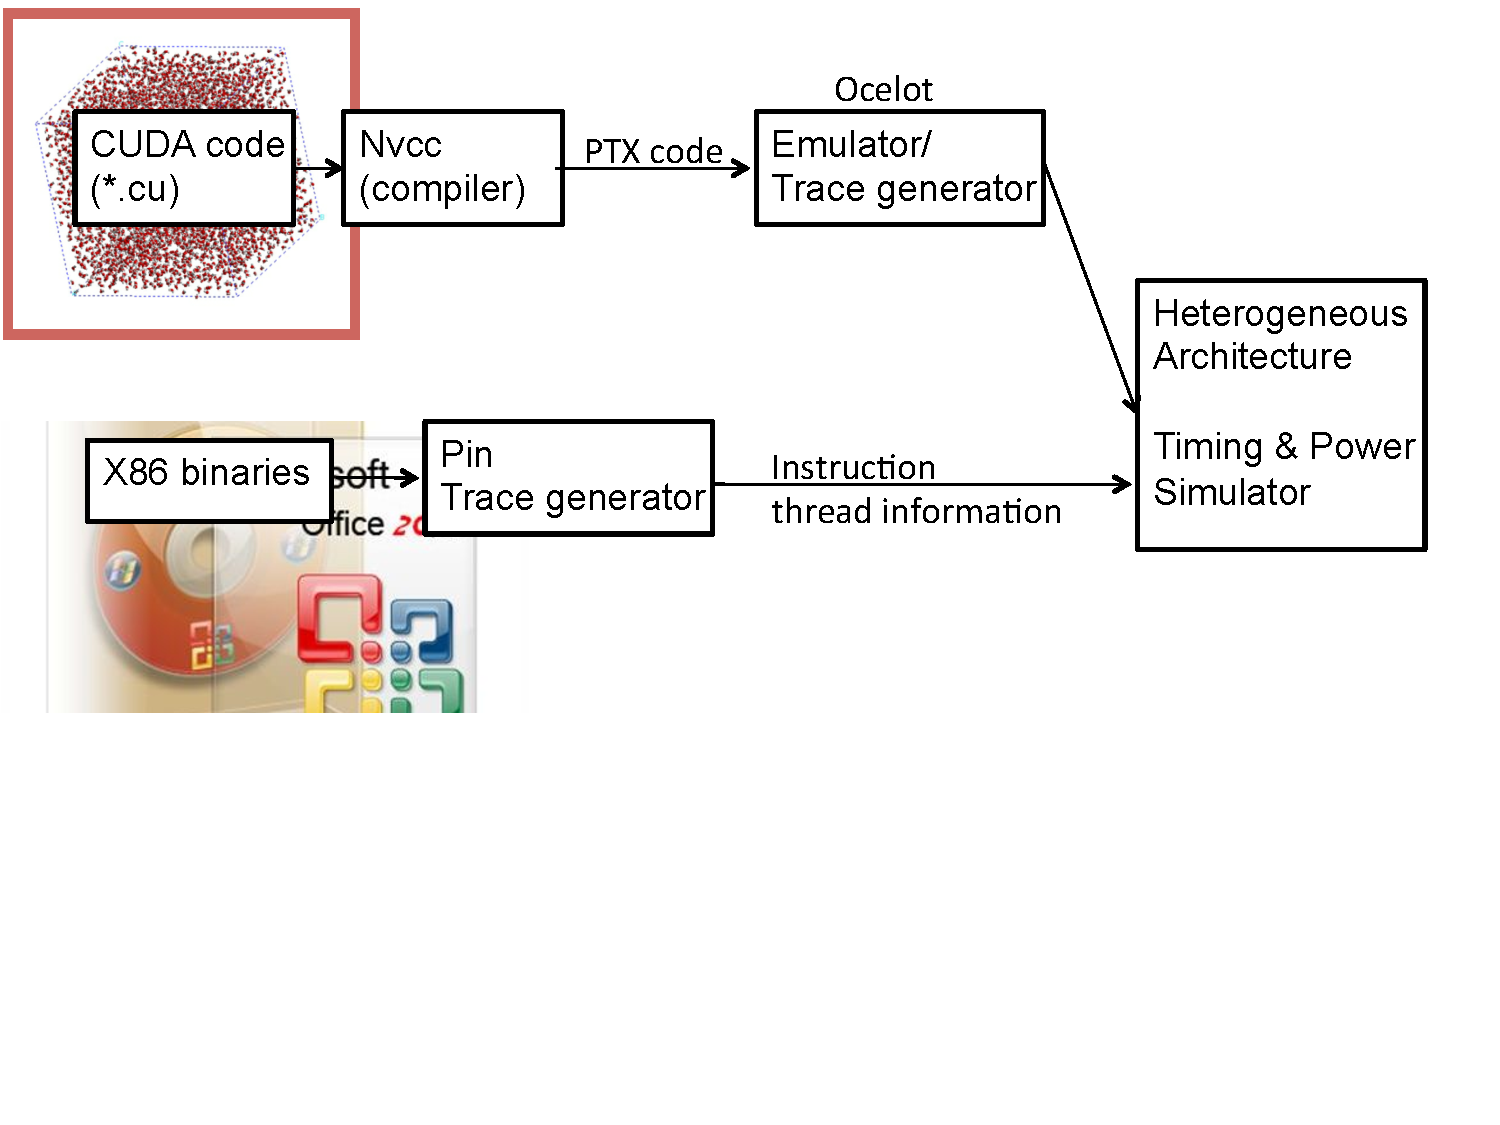
\includegraphics{figs/macsim_overview}
\caption{The overview of MacSim Simulator}
\label{fig:overview}
\end{figure*}


%%%%%%%%%%%%%%%%%%%%%%%%%%%%%%%%%%%%%%%%%%%%%%%%%%%%%%%%%%%%%%%%%%%%%%%%
%\section{Trace Generation}
%\label{sec:trace_generation}
%%%%%%%%%%%%%%%%%%%%%%%%%%%%%%%%%%%%%%%%%%%%%%%%%%%%%%%%%%%%%%%%%%%%%%%%



%%%%%%%%%%%%%%%%%%%%%%%%%%%%%%%%%%%%%%%%%%%%%%%%%%%%%%%%%%%%%%%%%%%%%%%%
\section{CPU (x86) Traces}
%%%%%%%%%%%%%%%%%%%%%%%%%%%%%%%%%%%%%%%%%%%%%%%%%%%%%%%%%%%%%%%%%%%%%%%%

\SIM includes a CPU (x86) trace generator which is based on Pin~\cite{pin}, a
binary instrumentation tool. Documentation regarding Pin can be found at
\urlc{http://www.pintool.org}. After installing Pin\footnote{Note that our
trace generator may not be backward/forward compatible with different Pin
versions. Currently, Pin 41150 revision (Jun 07, 2011) must be used.}, the x86
trace generator module has to be built. The command for doing so is:


\ignore{

CPU (x86) traces are generated with the aid of Pin~\cite{pin}, a
binary instrumentation tool.  Documentation regarding Pin can be found 
here \urlc{http://www.pintool.org}.  We provide
\cpu trace generator within \SIM repository. After installing
Pin\footnote{Note that our CPU trace generator may not be
  backward/forward compatible with the pin version. Currently, pin
  41150 revision (Jun 07, 2011) must be used.}, we need to build the
X86 trace generator module (trace\_generator.so), which can be simply
done with the following commands.
}



\begin{Verbatim}
cd toos/x86_trace_generator
make
\end{Verbatim}

\noindent
This will generate trace\_generator.so in the
tools/x86\_trace\_generator/obj-intel64 directory. x86
traces for \SIM can then be generated by running Pin with the generated module.


\begin{Verbatim}
pin -t trace_generator.so -- $BIN $ARGS (for single-threaded applications)
pin -t trace_generator.so -thread N -- $BIN $ARGS (for multi-threaded applications with N threads)
\end{Verbatim}


The following example shows the generation of traces for an execution of /bin/ls. 

\begin{Verbatim}
pin -t trace\_generator.so -- /bin/ls
\end{Verbatim}

\noindent The binary (ls) is actually executed on top of Pin and the
instructions executed by the binary are written to the trace file. The output
on the screen when generating traces for \textit{ls} is shown.



\begin{Verbatim}
pin -t trace_generator.so -- /bin/ls
-> Thread[0->0] begins.
-> Trace Generation Starts at icount 0
dump.txt_0.dump  pin.log  trace_0.raw  trace_generator.o  trace_generator.so  
xed_extractor.o  xed_extractor.so
-> Trace Generation Done at icount 475195
\end{Verbatim}

The trace generator generates two files (in case of a single threaded
    application) - Trace.txt and trace\_0.raw, in the current directory.
Section~\ref{sec:traceformat} provides details of the generated files.



%%%%%%%%%%%%%%%%%%%%%%%%%%%%%%%%%%%%%%%%%%%%%%%%%%%%%%%%%%%%%%%%%%%%%%%%
\section{GPU (PTX) Traces}
\label{sec:gpu_traces}
%%%%%%%%%%%%%%%%%%%%%%%%%%%%%%%%%%%%%%%%%%%%%%%%%%%%%%%%%%%%%%%%%%%%%%%%

GPU (PTX) traces are generated using GPUOcelot~\cite{ocelot}, a dynamic compilation
framework for heterogeneous systems. 


%%%%%%%%%%%%%%%%%%%%%%%%%%%%%%%%%%%%%%%%%%%%%%%%%%%%%%%%%%%%%%%%%%%%%%%%
\subsection{Installing Ocelot}
%%%%%%%%%%%%%%%%%%%%%%%%%%%%%%%%%%%%%%%%%%%%%%%%%%%%%%%%%%%%%%%%%%%%%%%%

Users can install Ocelot using the Ubuntu packages provided at the Google Code
page for Ocelot, or then can download the source and build and install Ocelot
themselves. Below is the sequence of commands to executed to build and install
from source. First, checkout a copy of Ocelot from its SVN repository.

\begin{Verbatim}
svn checkout http://gpuocelot.googlecode.com/svn/trunk/ gpuocelot
\end{Verbatim}


Then build Ocelot and the trace generator libraries.

\begin{Verbatim}
cd gpuocelot/ocelot; sudo ./build.py --install
cd gpuocelot/trace-generators; libtoolize; aclocal; autoconf; automake; ./configure; 
make; sudo make install
\end{Verbatim}


All libraries will be installed in the system library path directory
(\Verb+/usr/local/lib+). More detailed instructions for installing
Ocelot are available at the Google Code project page for Ocelot.


%%%%%%%%%%%%%%%%%%%%%%%%%%%%%%%%%%%%%%%%%%%%%%%%%%%%%%%%%%%%%%%%%%%%%%%%
\subsection{Generating Traces}
%%%%%%%%%%%%%%%%%%%%%%%%%%%%%%%%%%%%%%%%%%%%%%%%%%%%%%%%%%%%%%%%%%%%%%%%

CUDA executables targeted for trace generation must be linked against
libocelot.so and libocelotTrace.so. libocelot.so provides the functionality of
the CUDA runtime library (libcudart.so) and libocelotTrace.so contains the
trace generator for \SIM and tools provided by Ocelot.

To execute a binary linked against libocelot.so, a configuration file,
   \Verb+configure.ocelot+ (which is in JSON format), is required in the same
   directory as the binary. A copy of this file with some default settings can
   be obtained from the Ocelot source. To enable trace generation, open your
   copy of the configure.ocelot and add the pair \Verb+x86Trace: true+ on a new
   line under the trace member as shown below.  Make sure that there is a comma
   at the end of each pair that is not the last pair of a member.

\begin{Verbatim}
  trace: {
    database: "traces-ipdom/database.trace",
    memoryChecker: {
      enabled: true,
      checkInitialization: false
    },
    raceDetector: {
      enabled: true,
      ignoreIrrelevantWrites: true
    },
    cacheSimulator: {
      enabled: false,
    },
    branch: false,
    memory: false,
    x86Trace: true
  },
\end{Verbatim}

In addition to editing configure.ocelot, the following four environment
variables have to be set:

\begin{itemize}\itemsep2pt
\item TRACE\_PATH : directory to store generated traces. If not specified, current directory is used by default.
\item TRACE\_NAME : prefix used in the file name for generated traces. If not specified, "Trace" is used by default.
\item KERNEL\_INFO\_PATH : name of file that should contain kernel information (must be specified)
\item COMPUTE\_VERSION : compute capability (default 2.0)
\end{itemize}


Examples for setting up these environment variables are shown below.

\begin{Verbatim}
export TRACE_PATH="/storage/traces/"  # Create a trace directory in the /storage/traces
export KERNEL_INFO_PATH="kernel_info" # kernel_info has the kernel information
export COMPUTE_VERSION="2.0"          # Calculate occupancy based on compute capability 2.0
\end{Verbatim}

On executing the binary a kernel information file and one directory for each
kernel invocation by the binary containing the traces from the invocation are
generated in the directory pointed to by \Verb+TRACE\_PATH+. The kernel
information file contains the version of the traces generated and the path of
the trace configuration file for the traces generated for each kernel
invocation. The trace configuration file contains the number of warps, the
trace version, maximum number of thread blocks that can be assigned to each SM
and the id and starting information of each warp. More information regarding
the generated files can be found in Sections~\ref{sec:traceformat} and
~\ref{sec:kern_config}. 


\ignore
{
The kernel information file (kernel\_info) should contain the following
information: kernel name, register usage (per thread), and shared memory usage
(per thread).


\begin{Verbatim}
_Z9Memcpy_SWPfS_i 14 52 
\end{Verbatim}


Running CUDA application creates a directory with the kernel name, where traces 
are generated, and kernel\_config.txt which is a configuration used for MacSim.


\begin{Verbatim}
drwxr-xr-x   2 anonymous group 69632 Sep 00 22:03 _Z9Memcpy_SWPfS_i_0
-rw-r--r--   1 anonymous group    66 Sep 09 22:29 kernel_config.txt
\end{Verbatim}
}


%%%%%%%%%%%%%%%%%%%%%%%%%%%%%%%%%%%%%%%%%%%%%%%%%%%%%%%%%%%%%%%%%%%%%%%%
\section{Supporting Other Architectures}
%%%%%%%%%%%%%%%%%%%%%%%%%%%%%%%%%%%%%%%%%%%%%%%%%%%%%%%%%%%%%%%%%%%%%%%%

To support other ISAs such as ARM, a frontend simulator or a
functional emulator to provide the executed instruction stream is
necessary. Instructions in this stream can be translated by \SIM into
its internal RISC style micro-ops and simulated. Currently, plans for
supporting ARM ISA and OpenGL programs are in the pipeline.


%%%%%%%%%%%%%%%%%%%%%%%%%%%%%%%%%%%%%%%%%%%%%%%%%%%%%%%%%%%%%%%%%%%%%%%%
\section{Trace Formats}
\label{sec:traceformat}
%%%%%%%%%%%%%%%%%%%%%%%%%%%%%%%%%%%%%%%%%%%%%%%%%%%%%%%%%%%%%%%%%%%%%%%%

\paragraph{Note}

\textit{Although different trace generators use the same data structure for
storing instruction traces, the meaning of some of the members of this
common data structure is different in PTX traces. Note that efforts to
have different data structures for x86 and PTX traces for sake of
extensibility and clarity are underway.}


On successful trace generation, the x86 trace generator generates a
configuration file called Trace.txt and one Trace\_xx.raw file
(assuming that \Verb+TRACE\_PATH+ was set to "Trace") for each thread
of the application in the output directory. On the other hand, the PTX
trace generator generates a kernel information file and several
directories containing traces of individual kernel invocations. The
directory for each kernel invocation contains a Trace.txt file and one
Trace\_xx.raw file for each warp in the kernel.  Note that in case of
PTX kernels, one trace file is generated for each warp, there are no
per thread trace files. Further details regarding trace generation for
PTX kernels can be found in Section~\ref{sec:ptx_traces}. The purposes
of Trace.txt and Trace\_xx.raw are shown below and their formats are
explained in detail in subsequent sections.


\begin{itemize}\itemsep2pt
\item Trace.txt (info trace): contains information about the generated
  trace files (\#threads, trace type, ...).

\item Trace\_xx.raw (raw trace): contains instruction trace for a
  thread and is generated for each thread.\footnote{In case of GPU, a
    warp is mapped to a \SIM thread, where a warp consists of 32
    threads in CUDA.}
\end{itemize}



%%%%%%%%%%%%%%%%%%%%%%%%%%%%%%%%%%%%%%%%%%%%%%%%%%%%%%%%%%%%%%%%%%%%%%%%
\subsection{Trace.txt}
%%%%%%%%%%%%%%%%%%%%%%%%%%%%%%%%%%%%%%%%%%%%%%%%%%%%%%%%%%%%%%%%%%%%%%%%


\begin{figure*}[htb]
\centering
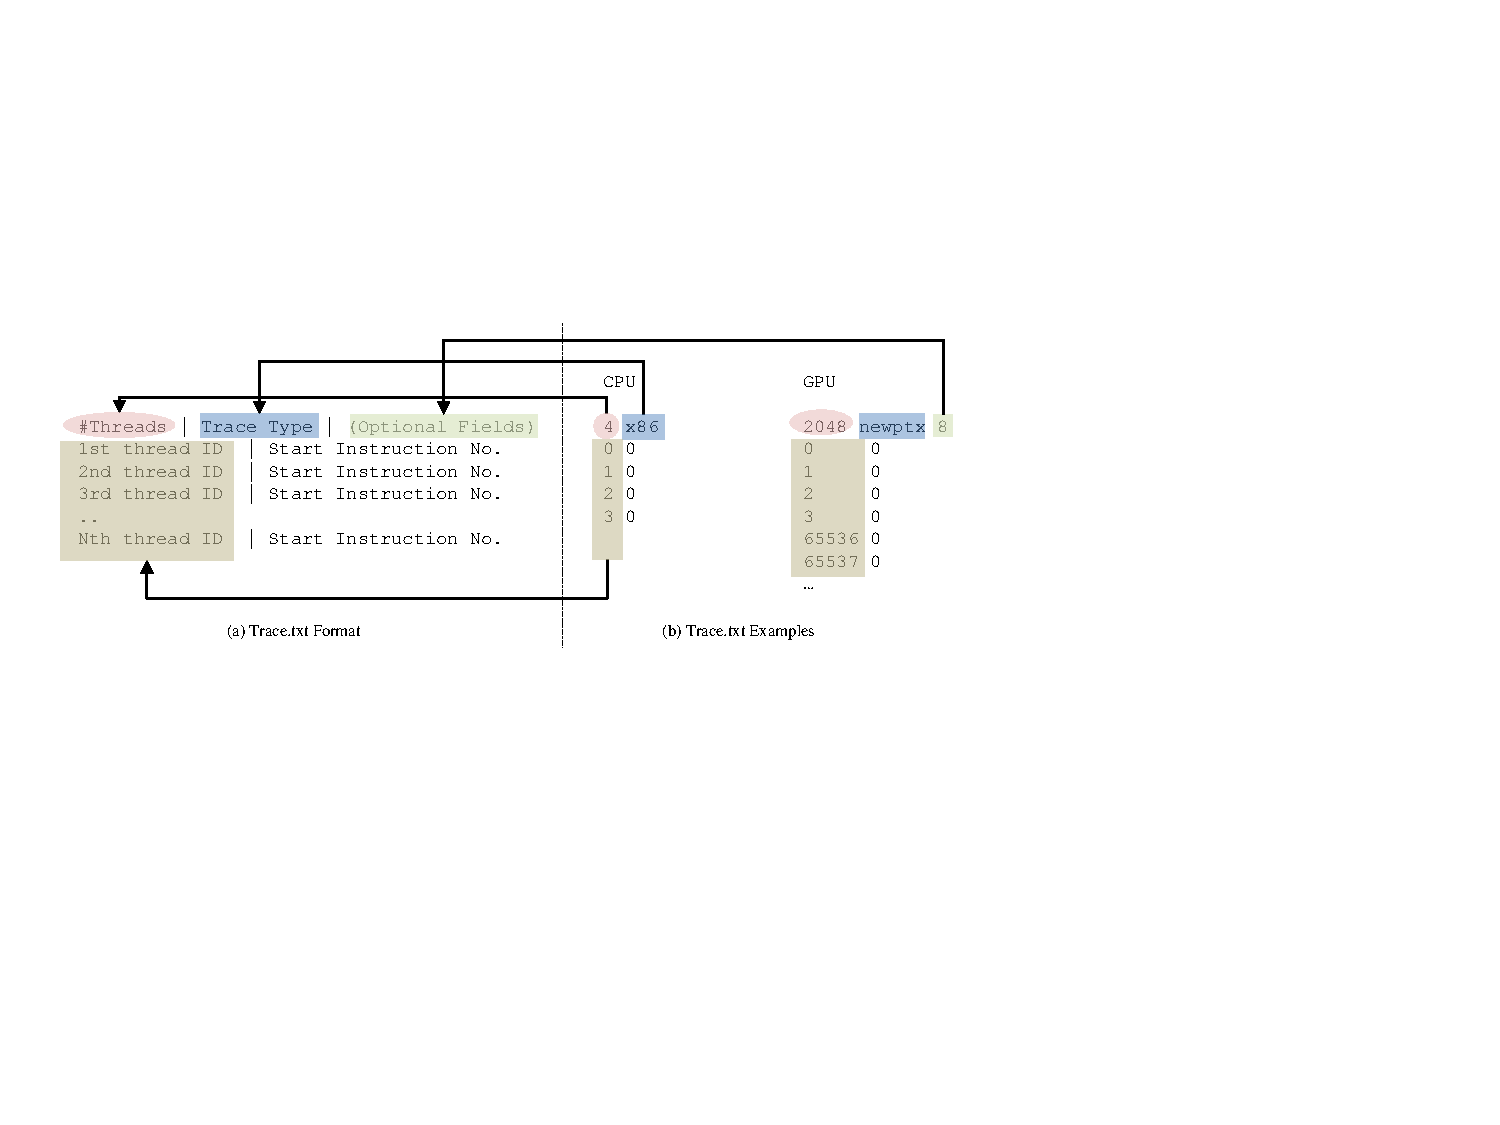
\includegraphics{figs/trace_format}
\caption{Trace.txt format.}
\label{fig:trace_format}
\end{figure*}


Figure~\ref{fig:trace_format} shows the format of Trace.txt and its CPU and GPU
examples.  As shown in Figure~\ref{fig:trace_format}-(a), the first line in
Trace.txt has different fields from the rest of the lines.

\begin{itemize}\itemsep2pt
\item \#Threads: indicates the number of threads for which traces have
  been generated, and this value is equal to the number of lines in
  the file excluding the first line.
\item Trace Type: indicates whether the generated traces are for an
  x86 application or a PTX kernel.
\item Optional Field(s): currently used for PTX traces only and
  indicates the number of thread blocks that can be assigned to a
  streaming multiprocessor(SM) core (occupancy).
\end{itemize}

From the second line onwards, there are two fields in each line:
thread id and start instruction number. For each thread, there is a
Trace\_<thread\_id>.raw file which contains the dynamic instruction
trace for the thread. Finally, start instruction number indicates when
each thread should be started in terms of the number of instructions
simulated for the main thread of the application. In a PTX kernel
since all warps are ready for execution at the launch of the kernel,
the start instruction number for all threads is zero. On the other
hand, for a x86 application, the start instruction is non-zero for all
threads except thread 0, which is the main (or parent) thread in the
application. This is because in most multi-threaded CPU applications,
main thread (thread id 0) spawns children threads.


In Figure~\ref{fig:trace_format}-(b), the CPU trace has four threads and its
type is set to x86. The ids of the threads are 0-3 with the corresponding trace
files being Trace\_0.raw$-$Trace\_3.raw . Thread 0 is ready at the start of
simulation, while Threads 1, 2 and 3 become ready when Thread 0 has fetched x,
  y and z instructions respectively.


In the GPU example, the number of traces files is 2048 since \#Threads
(representing \#Warps in case of GPUs) is 2048.  The optional field indicates
that eight thread blocks can be assigned to a SM core. 

For GPU traces, the id in the file encodes thread block information as
well. The warp id and thread block id can be decoded from this id as follows:

\begin{Verbatim}
warp_id  = id % (1 << 16)
block_id = id / (1 << 16)
\end{Verbatim}

\ignore{
In the GPU trace, thread ID is calculated by thread block ID * 65536 + warp ID (in a block). 
In the example, warps 0, 1, 2 and 3 are comprised of a thread block, and warps 65536, 65537, 65538
and 65539 forms another thread block.
}

%%%%%%%%%%%%%%%%%%%%%%%%%%%%%%%%%%%%%%%%%%%%%%%%%%%%%%%%%%%%%%%%%%%%%%%%
\subsection{Trace\_xx.raw}
%%%%%%%%%%%%%%%%%%%%%%%%%%%%%%%%%%%%%%%%%%%%%%%%%%%%%%%%%%%%%%%%%%%%%%%%

Trace\_xx.raw is generated for each thread/warp and contains the
dynamic instruction trace for the thread/warp in the binary
format. The structure/format for encoding instructions is the same in
both x86 and PTX traces and looks as follows (in order):


%trace format for an instruction in trace_xx.raw

\vspace{0.2in}
\begin{footnotesize}
\begin{tabular}{llll}
Type            & Size (Bytes) & Field                     & Description                                            \\ \hline
\Verb+uint8_t+  & 1            & \Verb+m_num_read_regs+    & number of source registers                             \\
\Verb+uint8_t+  & 1            & \Verb+m_num_dest_regs+    & number of destination registers                        \\
\Verb+uint8_t+  & 9            & \Verb+m_src[MAX_SRC_NUM]+ & source register IDs                                    \\
\Verb+uint8_t+  & 6            & \Verb+m_dst[MAX_DST_NUM]+ & destination register IDs                               \\
\Verb+uint8_t+  & 1            & \Verb+m_cf_type+          & branch type                                            \\
\Verb+bool+     & 1            & \Verb+m_has_immediate+    & indicates whether this instruction has immediate field \\
\Verb+uint8_t+  & 1            & \Verb+m_opcode+           & opcode                                                 \\
\Verb+bool+     & 1            & \Verb+m_has_st+           & indicates whether this instruction has store operation \\
\Verb+bool+     & 1            & \Verb+m_is_fp+            & indicates whether this instruction is a FP operation   \\
\Verb+bool+     & 1            & \Verb+m_write_flg+        & write flag                                             \\
\Verb+uint8_t+  & 1            & \Verb+m_num_ld+           & number of load operations                              \\
\Verb+uint8_t+  & 1            & \Verb+m_size+             & instruction size                                       \\
\Verb+uint32_t+ & 4            & \Verb+m_ld_vaddr1+        & load address 1                                         \\
\Verb+uint32_t+ & 4            & \Verb+m_ld_vaddr2+        & load address 2                                         \\
\Verb+uint32_t+ & 4            & \Verb+m_st_vaddr+         & store address                                          \\
\Verb+uint32_t+ & 4            & \Verb+m_instruction_addr+ & PC address                                             \\
\Verb+uint32_t+ & 4            & \Verb+m_branch_target+    & branch target address                                  \\
\Verb+uint8_t+  & 1            & \Verb+m_mem_read_size+    & memory read size                                       \\ 
\Verb+uint8_t+  & 1            & \Verb+m_mem_write_size+   & memory write size                                      \\
\Verb+bool+     & 1            & \Verb+m_rep_dir+          & repetition direction                                   \\
\Verb+bool+     & 1            & \Verb+m_actually_taken+   & indicates whether branch is actually taken             \\
\end{tabular}
\end{footnotesize}
\vspace{0.2in}


Note that the raw trace is compressed with zlib to reduce the sizes of
the generated trace files, and the size of each field is the size
before the compression.


%%%%%%%%%%%%%%%%%%%%%%%%%%%%%%%%%%%%%%%%%%%%%%%%%%%%%%%%%%%%%%%%%%%%%%%%
\subsection{kernel\_config.txt (only for PTX)}
\label{sec:kern_config}
%%%%%%%%%%%%%%%%%%%%%%%%%%%%%%%%%%%%%%%%%%%%%%%%%%%%%%%%%%%%%%%%%%%%%%%%

For PTX traces, as described in Section~\ref{sec:gpu_traces}, a directory is
created for each kernel invocation, where Trace.txt and Trace\_xx.raw are
generated. Since typical GPU applications usually invoke several kernels (or
    execute the same kernel repeatedly), PTX traces can have multiple kernel
directories. Thus, in order to simulate all invoked kernels for a GPU
application, the PTX trace generator creates kernel\_config.txt which contains
information of the invoked kernels.


\begin{Verbatim}
Contents of output directory after trace generation

ll /trace/ptx/parboil/bfs

drwxr-xr-x  4  4096 Sep 21 13:21 .
drwxr-xr-x 11  4096 Sep 13 18:02 ..
drwxr-xr-x  2  4096 Apr  7  2011 _Z17BFS_in_GPU_kernelPiS_P4int2S1_S_S_iS_ii_0
drwxr-xr-x  2  4096 Apr  7  2011 _Z26BFS_kernel_multi_blk_inGPUPiS_P4int2S1_S_S_S_S_iiS_S_S__0
-rw-r--r--  1   184 Apr  7  2011 kernel_config.txt

In kernel_config.txt

-1 newptx
/trace/ptx/parboil/bfs/_Z17BFS_in_GPU_kernelPiS_P4int2S1_S_S_iS_ii_0/Trace.txt
/trace/ptx/parboil/bfs/_Z26BFS_kernel_multi_blk_inGPUPiS_P4int2S1_S_S_S_S_iiS_S_S__0/Trace.txt
\end{Verbatim}


As shown above, all the invoked kernels are enumerated in kernel\_config.txt.
The first line indicates that this is a wrapper file which points to (multiple)
  trace.txt files, one for each kernel invocation. \SIM reads and simulates the
  traces sequentially, one kernel at a time.  In the above example (bfs),
  kernel\_config.txt indicates that there are two different kernels in bfs,
  each of which was invoked once. When running a GPU simulation, the path to
  the kernel\_config.txt file is specified trace\_file\_list
  (Section~\ref{sec:run}).  Also, we can simulate specific kernels
  by modifying the kernel\_config.txt file.

%%%%%%%%%%%%%%%%%%%%%%%%%%%%%%%%%%%%%%%%%%%%%%%%%%%%%%%%%%%%%%%%%%%%%%%%
\subsection{Translation into micro-ops}
%%%%%%%%%%%%%%%%%%%%%%%%%%%%%%%%%%%%%%%%%%%%%%%%%%%%%%%%%%%%%%%%%%%%%%%%

During simulation, each instruction in a \emph{raw trace} file is
converted into one or more micro-ops internally. \SIM stores such
decoded micro-uops in the MacSim-specific structure shown in in
Table~\ref{table:trace_uops}.

\begin{table*}[htb]
\begin{footnotesize}
\begin{center}
\caption{MacSim-specific data structure for micro-ops.}
\label{table:trace_uops}
\begin{tabular}{|l|l|l|} 
\hline
Type      & Variable                 & Description \\ \hline \hline
uint8\_t  & m\_opcode                & opcode \\ \hline
Uop\_Type & m\_op\_type              & type of operation \\ \hline
Mem\_Type & m\_mem\_type             & type of memory instruction \\ \hline
Cf\_Type  & m\_cf\_type              & type of control flow instruction \\ \hline
Bar\_Type & m\_bar\_type             & type of barrier caused by instruction \\ \hline
uns       &   m\_num\_dest\_regs     & number of destination registers written \\ \hline
uns       &   m\_num\_src\_regs      & number of source registers read \\ \hline
uns       &   m\_mem\_size           & number of bytes read/written by a memory instruction \\ \hline
uns       &   m\_inst\_size          & instruction size \\ \hline
Addr      &   m\_addr                & PC address  \\ \hline
reg\_info\_s&   m\_srcs[MAX\_SRCS]   & source register information \\ \hline
reg\_info\_s&   m\_dests[MAX\_DESTS] & destination register information \\ \hline
Addr      &   m\_va;                 & virtual address \\ \hline
bool      &   m\_actual\_taken       & branch actually taken \\ \hline
Addr      &   m\_target              & branch target address \\ \hline
Addr      &   m\_npc                 & next PC address  \\ \hline
bool      &   m\_pin\_2nd\_mem       & has second memory operation \\ \hline
inst\_info\_s& *m\_info              & pointer to the instruction hash table  \\ \hline
int       &   m\_rep\_uop\_num       & repeated uop number \\ \hline
bool      &   m\_eom                 & end of macro \\ \hline
bool      &   m\_alu\_uop            & ALU uop  \\ \hline
uint32\_t  &   m\_active\_mask       & active mask \\ \hline
uint32\_t  &   m\_taken\_mask        & branch taken mask \\ \hline
Addr      &   m\_reconverge\_addr    & address of reconvergence \\ \hline
bool      &   m\_mul\_mem\_uops      & multiple memory transactions \\ \hline

\end{tabular}
\end{center}
\end{footnotesize}
\end{table*}

\ignore{
The following shows the data structure for micro-uops. 


\begin{Verbatim}
  uint8_t      m_opcode;        /**< opcode */
  Uop_Type     m_op_type;       /**< type of operation */
  Mem_Type     m_mem_type;      /**< type of memory instruction */
  Cf_Type      m_cf_type;       /**< type of control flow instruction */ 
  Bar_Type     m_bar_type;      /**< type of barrier caused by instruction */
  uns          m_num_dest_regs; /**< number of destination registers written */
  uns          m_num_src_regs;  /**< number of source registers read */
  uns          m_mem_size;      /**< number of bytes read/written by a memory instruction */
  uns          m_inst_size;     /**< instruction size */
  Addr         m_addr;          /**< pc address */ 
  reg_info_s   m_srcs[MAX_SRCS]; /**< source register information */
  reg_info_s   m_dests[MAX_DESTS]; /**< destination register information */
  Addr         m_va;            /**< virtual address */
  bool         m_actual_taken;  /**< branch actually taken */
  Addr         m_target;        /**< branch target address */
  Addr         m_npc;           /**< next pc address */ 
  bool         m_pin_2nd_mem;   /**< has second memory operation */
  inst_info_s *m_info;          /**< pointer to the instruction hash table */ 
  int          m_rep_uop_num;   /**< repeated uop number */
  bool         m_eom;           /**< end of macro */
  bool         m_alu_uop;       /**< alu uop */ 
  // GPU simulation
  uint32_t     m_active_mask;   /**< active mask */
  uint32_t     m_taken_mask;    /**< branch taken mask */
  Addr         m_reconverge_addr; /**< address of reconvergence */
  bool         m_mul_mem_uops;  /**< multiple memory transactions */
\end{Verbatim}

}

% LocalWords:  GPU PTX gpuocelot

%%%%%%%%%%%%%%%%%%%%%%%%%%%%%%%%%%%%%%%%%%%%%%%%%%%%%%%%%%%%%%%%%%%%%%%%%%%%%%%%%%%%%%

\ignore{
\begin{table*}[htb]
\begin{footnotesize}
\begin{center}
\caption{MacSim trace format.}
\label{table:trace_format}
\begin{tabular}{|l|l|} 
\hline
Type               & Description \\ \hline 
uint8\_t           & number of source registers \\ \hline
uint8\_t           & number of destination registers \\ \hline
uint8\_t[9]        & source register IDs \\ \hline
uint8\_t[6]        & destination register IDs \\ \hline
uint8\_t           & branch type \\ \hline
bool               & indicates whether this instruction has immediate field \\ \hline
uint8\_t           & opcode \\ \hline
bool               & indicates whether this instruction has store operation \\ \hline
bool               & indicates whether this instruction is FP operation \\ \hline
bool               & write flag \\ \hline
uint8\_t           & number of load operations \\ \hline
uint8\_t           & instruction size \\ \hline
uint32\_t          & load address 1 \\ \hline
uint32\_t          & load address 2 \\ \hline
uint32\_t          & store address \\ \hline
uint32\_t          & PC address \\ \hline
uint32\_t          & branch target address \\ \hline
uint32\_t          & memory read size \\ \hline
uint8\_t           & memory write size \\ \hline
uint8\_t           & repetition direction  \\ \hline
uint8\_t           & indicates whether branch is actually taken \\ \hline

\end{tabular}
\end{center}
\end{footnotesize}
\end{table*}
}

\ignore{
\begin{table*}[htb]
\begin{footnotesize}
\begin{center}
\caption{MacSim trace format.}
\label{table:trace_format}
\begin{tabular}{|l|l|l|l|l|l|l|l|l|l|l|l|l|l|l|l|} 
\hline
nSR & nDR & SR\_IDs & DR\_IDs & BrType & bImm & Opcode & bStore & bFP & WF & nLD  \\ \hline \hline
InstSize & LAddr\_1 & LAddr\_2 & SAddr & PCAddr & BrAddr & MemRSize & MemWSize & RepDir & BrActT & \\ \hline
\end{tabular}
\end{center}
\end{footnotesize}
\end{table*}

Tables~\ref{table:trace_format} and ~\ref{table:trace_desc} show the trace
format for each instruction and the description of each field, respectively.
}




%
\clearpage
\section{Macsim Installation and Run}

\subsection{Download}

\SIM source code is maintained using the subversion. 
You can check out the \SIM copy by

\smallskip
\begin{lstlisting}
svn co https://svn.research.cc.gatech.edu/macsim/trunk macsim-readonly --username readonly
\end{lstlisting}
\smallskip


\subsection{Wiki and Other Supports}

We manage the google project page in the following url:

\smallskip
\begin{lstlisting}
http://code.google.com/p/macsim/
\end{lstlisting}
\smallskip


\subsection{Build Requirement}

\SIM requires following to build properly.

\begin{description}

  \item[Operating System] Currently, we only support linux
  distributions. Tested systems are as follows:

  \smallskip
  \begin{lstlisting}
  Ubuntu
  Redhat (todo)
  \end{lstlisting}
  \smallskip

  \item[Compiler] Any compiler that can supports the C++0x (or C++11)
  standard library. Currently, we tested follwing compilers:
        
  \smallskip 
  \begin{lstlisting}
  gcc   
  icc (todo)
  \end{lstlisting} 
  \smallskip

  \item[Autotools] - You need to have autotools (automake, autoconf,
  ...) version 2.65 or higher. You can install autotools by

  \smallskip
  \begin{lstlisting}
  Ubuntu: apt-get install autotools-dev automake autoconf
  Redhat: todo
  \end{lstlisting}
  \smallskip


\end{description}

\ignore{
\subsection{Directory Structure}

This section explains the directory structure of \SIM simulator.

\smallskip
\begin{lstlisting}
macsim/
  tag/ branch/ trunk/
\end{lstlisting}
\smallskip

\textit{Tag} directory has tagged version of \SIM
simulators. \textit{Branch} directory is for diverged \SIM, which is
currently empty. \textit{Trunk} directory is current working directory
for \SIM.

Following is more detailed information about \textit{Trunk} directory.

\smallskip
\begin{lstlisting}
trunk/
  bin/ def/ doc/ params/ scripts/ src/ tools/
\end{lstlisting}
\smallskip

\textit{Bin} directory contains the \SIM binary after the building
process. \textit{def} directory has knob (Section~\ref{sec:knob}) and
statistics (Section~\ref{sec:stat}) definitions. \textit{doc} has the
documentation. \textit{scripts} includes several scripts files that
are using during the building process. \textit{src} contains all
source files. \textit{tools} has several useful tools.
\ignore{ (Section~\ref{sec:tool}) }
}





\subsection{Installation}

The GNU Autotools (automake, autoconf) have been used for building
\SIM simulator. After initial check out of the \SIM copy, following commands are necessary.

\smallskip
\begin{lstlisting}
aclocal 
automake 
--add-missing 
autoconf 
./configure 
make
\end{lstlisting}
\smallskip

You can combine above commands in a line:

\smallskip
\begin{lstlisting}
aclocal && automake --add-missing && autoconf && ./configure && make
\end{lstlisting}
\smallskip

We provide autogen.sh script file to simplify the building process.

\smallskip
\begin{lstlisting}
./autogen.sh
make
\end{lstlisting}
\smallskip

The binary \textit{macsim} will be generated in the
\textit{trunk/bin/} directory.





\subsection{Build Types}

We provide three different build types.

\begin{itemize}
  \item opt : default, optimized version (-O3 flag)
  \item dbg : debug version (-g3 flag)
  \item gpf : gprof version (-pg flag)
\end{itemize}

To build a certain type, you need to specify the option
after \textit{make} command. For example,

\smallskip
\begin{lstlisting}
make opt
make dbg
make gpf
\end{lstlisting}
\smallskip





\subsection{How To Run \SIM}

To run \textit{macsim} binary, two additional files are required in
the same directory.

\begin{itemize}
  \item params.in - defines architectural parameters that will
  overwrite the default value.

  \item trace\_file\_list - defines the number of traces to run and
  the path of each trace
\end{itemize}

\subsubsection{params.in}

We provide sample parameter files for various architectures (Intel
CPUs, NVIDIA GPUs, ...) in
the \textit{macsim-top/trunk/params}. Following is sample content of
params.in file.

\smallskip
\begin{lstlisting}
# Simulation Configuration
num_sim_cores 1
num_sim_small_cores 0
num_sim_medium_cores 0
num_sim_large_cores 1
core_type ptx
large_core_type x86
cpu_frequency 4
gpu_frequency 1.5
sim_cycle_count 0
max_insts 500000000
heartbeat_interval 1000000
forward_progress_limit 50000


# Common Core Configuration
fetch_policy rr
mt_no_fetch_br 1
one_cycle_exec 0
\end{lstlisting}
\smallskip

The first literal is the name of parameter and the second literal is a
value that will overwrite the default value. Section~\ref{sec:knob}
details how to add, modify, and use these parameters.


\subsubsection{trace\_file\_list}

Following is the content of a sample trace\_file\_list.

\smallskip
\begin{lstlisting}
2
/trace/ptx/cuda2.2/FastWalshTransform/kernel_config.txt
/trace/ptx/cuda2.2/BlackScholes/kernel_config.txt
\end{lstlisting}
\smallskip

The first line is the number of traces that \SIM will run and
following lines are the path of each traces. Each top level trace
configuration file contains various information. Following is the
content of a top-level trace information file.


\smallskip
\begin{lstlisting}
1 x86
0 0
\end{lstlisting}
\smallskip

In the first line, the first number indicates the number of threads in
the application and second literal specifies the type of the
application. Trailing lines are the information of each thread
({thread id}, {thread starting point in terms of the instruction count
of the main thread (thread 0)}). Section~\ref{sec:traceformat}
describes the detail of the trace file format.



\subsubsection{Run}

The following is the sample command lines to run \SIM simulator.

\smallskip
\begin{lstlisting}
./macsim [additional commands]
./macsim --l2_assoc=8 --stdout=stdout --stderr=stderr
./macsim --l1_assoc=4 
\end{lstlisting}
\smallskip



\subsubsection{Runnint Repeat Traces} 

% LocalWords:  Macsim svn macsim readonly username params src Autotools aclocal
% LocalWords:  automake autoconf autogen dbg gpf gprof CPUs NVIDIA GPUs num sim
% LocalWords:  ptx cpu gpu insts rr br Wiki google url linux Redhat todo gcc
% LocalWords:  icc autotools dev stdout stderr

%


% LocalWords:  macsim num sim SMT multi pre NVIDIA params GeForce gtx GTX ptx
% LocalWords:  GeForece Multipe SMs appl GPU cpu gpu CUDA GPUOcelot RCD mc GHz
% LocalWords:  precharge rowbuffer FRFCFS MCs FCFS Prefetching prefetcher alloc
% LocalWords:  icache Microarchitecture bp dir mech gshare isched msched fsched
% LocalWords:  FP io ooo rr th sched const mem

%
\clearpage
\section{CPU-GPU Heterogeneous Simulation}




% LocalWords:  GPU


\clearpage
\section{The Knobs and Statistics}


Describe knob variables and statistics.






%%%%%%%%%%%%%%%%%%%%%%%%%%%%%%%%%%%%%%%%%%%%%%%%%%%%%%%%%%%%%%%%%%%%%%%%
\chapter{Simulation Statistics}
\label{sec:stat}
%%%%%%%%%%%%%%%%%%%%%%%%%%%%%%%%%%%%%%%%%%%%%%%%%%%%%%%%%%%%%%%%%%%%%%%%

A simple framework for collecting statistics (hereafter referred to as stats)
  during simulation is provided.  Stats can be either global (includes
      data from all cores) or per core.

%%%%%%%%%%%%%%%%%%%%%%%%%%%%%%%%%%%%%%%%%%%%%%%%%%%%%%%%%%%%%%%%%%%%%%%%
\section{Stat Types}
%%%%%%%%%%%%%%%%%%%%%%%%%%%%%%%%%%%%%%%%%%%%%%%%%%%%%%%%%%%%%%%%%%%%%%%%

The following stat types are supported:

\begin{description}

  \item [COUNT] for counting the number of occurances of an event. Eg. number
  of cache hits. 

  \item [RATIO] for calculating the ratio of number of occurances of one event
  over another. Eg. (number of cache hits / number of cache accesses) i.e.,
  cache hit ratio.

  \item [DIST]  for calculating the proportion of each event in a group of
  events.  \ignore{for defining a group of related events and calculating the
    number of occurances of each event in the group as a percent of the sum of
      the number of occurances of all events in the group.}  Eg. If the user
      wants to know what percent of L1 data cache accesses (in a 2-level
          hierarchy) resulted in L1 hits, L2 hits or memory accesses, then the
      user should define a distribution consisting on three events - L1 hits,
      L2 hits and L2 misses  - and update the counter for each event correctly. 

\end{description}


Note that a simulation will output two values for each stat. One is the
raw value i.e. the number of occurances of the event associated with the
stat and the other value is the value calculated based on the type
of the stat.


%%%%%%%%%%%%%%%%%%%%%%%%%%%%%%%%%%%%%%%%%%%%%%%%%%%%%%%%%%%%%%%%%%%%%%%%
\section{Adding a new stat}
%%%%%%%%%%%%%%%%%%%%%%%%%%%%%%%%%%%%%%%%%%%%%%%%%%%%%%%%%%%%%%%%%%%%%%%%

New stats can be defined by adding DEF\_STAT statements to any of the
\textit{*.stat.def} files in the \textit{trunk/def/} directory or by creating a
\textit{.stat.def} file including the definitions in the \textit{trunk/def/}
directory.  To define a per core statistic specify PER\_CORE at the
end of each DEF\_STAT statement below.



\begin{description}

\item[COUNT Stat:] \Verb+ +

\Verb+DEF_STAT(STAT_NAME, COUNT, NO_RATIO [, PER_CORE])+

Eg: 
\begin{Verbatim}
DEF_STAT(INST_COUNT_TOT, COUNT, NO_RATIO)
DEF_STAT(INST_COUNT, COUNT, NO_RATIO, PER_CORE)
\end{Verbatim}

\item[RATIO Stat:] \Verb+ +

\Verb+DEF_STAT(STAT_NAME, RATIO, BASE_STAT_NAME [, PER_CORE])+


In addition to defining the RATIO stat itself, a base stat of type COUNT has to
be defined as well. The value of the base stat is used as the denominator in
calculating the ratio. 

Eg: 
\begin{Verbatim}
DEF_STAT(DISPATCHED_INST, COUNT, NO_RATIO)
DEF_STAT(DISPATCH_WAIT, RATIO, DISPATCHED_INST)
\end{Verbatim}

\item[DIST Stat:] \Verb+ +

\begin{Verbatim}
DEF_STAT(STAT_NAME_START, DIST, NO_RATIO [, PER_CORE])
DEF_STAT(STAT_NAME, COUNT, NO_RATIO [, PER_CORE])*
DEF_STAT(STAT_NAME_END, DIST, NO_RATIO [, PER_CORE])
\end{Verbatim}

The definition of a DIST stat requires at least two stats.

Eg: 
\begin{Verbatim}
DEF_STAT(SCHED_FAILED_REASON_SUCCESS, DIST, NO_RATIO, PER_CORE)
DEF_STAT(SCHED_FAILED_OPERANDS_NOT_READY, COUNT, NO_RATIO, PER_CORE)
DEF_STAT(SCHED_FAILED_NO_PORTS, DIST, NO_RATIO, PER_CORE)
\end{Verbatim}

\end{description}


%%%%%%%%%%%%%%%%%%%%%%%%%%%%%%%%%%%%%%%%%%%%%%%%%%%%%%%%%%%%%%%%%%%%%%%%
\section{Updating Stats}
%%%%%%%%%%%%%%%%%%%%%%%%%%%%%%%%%%%%%%%%%%%%%%%%%%%%%%%%%%%%%%%%%%%%%%%%


Macros are provided to update the value of stats. STAT\_EVENT and
STAT\_EVENT\_M increment and decrement the value of a global stat by 1 and take
the name of the stat to be updated as their argument.  STAT\_EVENT\_N is used
to increment the value of a global stat by more than than 1. It takes the name
of the stat to be incremented and the value to be added as its arguments.
STAT\_CORE\_EVENT and STAT\_CORE\_EVENT\_M increment and decrement the value of
a per core stat by 1. These take core id and the name of the stat to be
incremented/decremented as their parameters. For example,

\begin{Verbatim}
STAT_EVENT(INST_COUNT_TOT); // increments global stat INST_COUNT_STAT by 1
STAT_EVENT_N(INST_COUNT_TOT, 2); // increments global stat INST_COUNT_STAT by 2
STAT_EVENT_M(INST_COUNT_TOT); // decrements global stat INST_COUNT_STAT by 1
STAT_CORE_EVENT(0, INST_COUNT); // increments stat INST_COUNT for core 0 by 1
\end{Verbatim}



%%%%%%%%%%%%%%%%%%%%%%%%%%%%%%%%%%%%%%%%%%%%%%%%%%%%%%%%%%%%%%%%%%%%%%%%
\section{Simulation output}
%%%%%%%%%%%%%%%%%%%%%%%%%%%%%%%%%%%%%%%%%%%%%%%%%%%%%%%%%%%%%%%%%%%%%%%%

At the end of a simulation several files with the extension stat.out are
generated, these files include the stat values at the end of the
simulation. As mentioned, for each stat two values are generated, one is the
raw stat value and other is a value calculated based on the type of the
stat. For simulations with multiple applications, multiple sets of stat files
are generated. Each simulated application is assigned an integer id (these ids
    are assigned according to the order in which the applications appear in the
    trace\_file\_list), when an application terminates (for the first time,
      note that applications may be repeated), stat files suffixed with the the
    id of the application, i.e.  *.stat.out.<appl\_id>, are generated. These
    stat files contain the value of the stats until that point in the
    simulation. At the end of the simulation, *.stat.out files are generated as
    usual.



%%%%%%%%%%%%%%%%%%%%%%%%%%%%%%%%%%%%%%%%%%%%%%%%%%%%%%%%%%%%%%%%%%%%%%%%
\section{Important Stats}
%%%%%%%%%%%%%%%%%%%%%%%%%%%%%%%%%%%%%%%%%%%%%%%%%%%%%%%%%%%%%%%%%%%%%%%%

\TODO{better to remove this, adding more stats will be difficult}

\begin{table}[htb]
\begin{footnotesize}
\begin{center}
\caption{Important Stats.} 
\label{table:stats}
\begin{tabular}{|l||l|c|l|}
\hline 
INST\_COUNT\_TOT            & \# of instructions                                    &      & general.stat.out \\ \hline 
INST\_COUNT\_CORE\_[0-11]   & \# of instructions in only the specificed core [0-11] & core & general.stat.out \\ \hline 
CYC\_COUNT\_TOT             & simulated cycles                                      &      & general.stat.out \\ \hline 
CYC\_COUNT\_CORE\_[0-11]    & simulated cycles in only the specificed core [0-11]   &      & general.stat.out \\ \hline 
CYC\_COUNT\_X86             & simulated cycles for x86 only                         &      & general.stat.out \\ \hline 
CYC\_COUNT\_PTX             & simulated cycles for ptx only                         &      & general.stat.out \\ \hline \hline 
                            & \# of fp instructions                                 &      &                  \\ \hline 
                            & \# of int instructions                                &      &                  \\ \hline 
                            & \# of load instructions                               &      &                  \\ \hline  
                            & \# of store instructions                              &      &                  \\ \hline  
BP\_ON\_PATH\_CORRECT       & \# of correctly predicted branches (DIST)             & core & bp.stat.def      \\ \hline  
BP\_ON\_PATH\_MISPREDICT    & \# of mis-predicted branches (DIST)                   & core & bp.stat.def      \\ \hline  
BP\_ON\_PATH\_MISFETCHT     & \# of mis-fetch branches (BTB MISS)(DIST)             & core & bp.stat.def      \\ \hline  
ICACHE\_HIT, ICACHE\_MISS   & \# of I-cache hitt,miss (DIST)                        &      & memory.stat.def  \\ \hline  
L[1-3]\_HIT\_CPU            & \# of l[1-3]cache hits from CPU                       &      & memory.stat.def  \\ \hline 
L[1-3]\_HIT\_GPU            & \# of l[1-3]cache hits from GPU                       &      & memory.stat.def  \\ \hline 
L[1-3]\_MISS\_CPU           & \# of l[1-3]cache misses from CPU                     &      & memory.stat.def  \\ \hline 
L[1-3]\_MISS\_GPU           & \# of l[1-3]cache misses from GPU                     &      & memory.stat.def  \\ \hline  \hline 
AVG\_MEMORY\_LATENCY        & average memory latency                                &      & memory.stat.def  \\ \hline \hline 
TOTAL\_DRAM                 & \# of DRAM accesses                                   &      & memory.stat.def  \\ \hline  
TOTAL\_DRAM\_READ           & \# of DRAM reads                                      &      & memory.stat.def  \\ \hline  
TOTAL\_DRAM\_WB             & \# of DRAM write backs                                &      & memory.stat.def  \\ \hline  
                            & \# of register reads                                  &      &                  \\ \hline  
                            & \# of register writes                                 &      &                  \\ \hline   \hline 
COAL\_INST, UNCOAL\_INST    & coalesced/uncoalesced mem requests (DIST)             &      & memory.stat.def  \\ \hline 




\end{tabular}
\end{center}
\end{footnotesize}
\end{table} 



\chapter{Source Organization}


\TODO{check this, i'm not sure what is included in the copy that be available
  publically} 

The top-level source directory of \SIM contains several directories, README and
INSTALL files and files required for building \SIM using autotools. Below is a
brief description of the contents of the top-level source directory of \SIM.


\begin{description}\firmlist

\item [bin] Build output directory.

\item [def] Contains definitions of parameters (see Sections~\ref{sec:run}
    and~\ref{sec:knob}) and events for statistics (see Section~\ref{sec:stat}).

\item [doc] Contains \SIM documentation.

\item [params] Contains sample parameter (see Sections~\ref{sec:run}
    and~\ref{sec:knob}) configuration files.

\item [scripts] Contains scripts used in build of \SIM.

\item [src] Contains \SIM source files (.cc and .h files).

\item [tools] Contains x86 trace generator and trace reader.

\item [README, INSTALL] README and INSTALL files containing proceduce to build
and run \SIM and patch \SIM to make it usable as a SST component (see
    Section~\ref{sec:sst}).

\item [autogen.sh] Script file to generate makefile to build \SIM.

\item [configure.in aclocal.m4 Makefile.am Makefile.in] Files required by
autotools to generate makefile to build \SIM.

\end{description}



Table~\ref{table:file_list} shows the list of source file and the purpose/content of
each file.

\begin{table}[htb]
\begin{footnotesize}
\begin{center}
\caption{Source files and their purpose/content}
\label{table:file_list}
\begin{tabular}{|c||c|}
\hline 
File(s)                                                      & Purpose                            \\ \hline
frontend.cc/h, fetch\_factory.cc/h, bp*.cc/h                 & Fetch stage                        \\ \hline 
allocate*.cc/h, rob*.cc/h, map.cc/h                          & Decode and Allocate stages         \\ \hline
schedule*.cc/h                                               & Schedule stage                     \\ \hline 
exec.cc/h                                                    & Execution stage                    \\ \hline 
retire.cc/h                                                  & Retire stage                       \\ \hline       
port.cc/h, cache.cc/h dram.cc/h, memory*.cc/h, \\ 
memreq\_info.cc/h, readonly\_cache.cc/h, \\ 
sw\_managed\_cache.cc/h                                      & Memory system                      \\ \hline 
pref*.cc/h                                                   & Prefetchers                        \\ \hline
trace\_read.cc/h inst\_info.h                                & Reading traces                     \\ \hline
core.cc/h                                                    & Class representing a core being simulated \\ \hline
process\_manager.cc/h                                        & Process Manager/thread scheduler   \\ \hline 
uop.cc/h                                                     & Uop structure and related enums    \\ \hline
\multirow{2}{*}{macsim.cc/h}                                 & Class containing pointers to the simulated cores, NoC, \\
                                                               memory system, knobs and other objects \\ \hline
knob.cc/h                                                    & Classes for supporting knobs       \\ \hline
statistics.cc/h                                              & Classes for supporting knobs       \\ \hline
factory\_class.cc/h                                          & Implementation of different factory classes                          \\ \hline
bug\_detector.cc/h                                           & Class useful for debugging forward progress errors happen             \\ \hline
utils.cc/h                                                   & Utility classes and functions      \\ \hline
debug\_macros.h                                              & Macros for debugging               \\ \hline
assert\_macros.h                                             & Macros for assert statements with debug information                  \\ \hline
global*.h                                                    & Forward declarations and typedefs  \\ \hline

\end{tabular}
\end{center}
\end{footnotesize}
\end{table}



\ignore
{
\begin{table}[htb]
\begin{footnotesize}
\begin{center}
\caption{Pipeline stage and the corresponding source files.}
\label{table:pipeline}
\begin{tabular}{|c||c|}
\hline 
pipeline stage         & file names                                             \\ \hline \hline 
main simulator         & macsim.cc, core.cc                                     \\ \hline 
fetch stage            & frontend.cc, fetch\_factory.cc, bp.cc, bp\_*.cc        \\ \hline 
decode stage           & allocate.cc                                            \\ \hline 
allocate stage         & allocate.cc, allocate\_*.cc, rob.cc, rob\_*.cc, map.cc \\ \hline 
schedule stage         & schedule.cc, schedule\_*.cc                            \\ \hline 
execution stage        & exec.cc                                                \\ \hline 
retire stage           & retire.cc                                              \\ \hline 
memory system          & port.cc, cache.cc *\_cache.cc, dram.cc, memory.cc      \\ \hline \hline
other supporting files & statistics.cc, bug\_detector.cc                        \\ \hline \hline 
process manager        & process\_manager.cc                                    \\ \hline 
\end{tabular}
\end{center}
\end{footnotesize}
\end{table}
}




%
\clearpage
\section{SST-Macsim}

Macsim is a part of SST simulation framework.

\subsection{How to install SST}

\subsection{How to install \SIM in SST}

Check out the svn copy of \SIM in \textit{sst-top/sst/elements} and
apply a patch. Then, compile SST again.

\smallskip
\begin{lstlisting}
cd sst-top/sst/elements
svn co https://svn.research.cc.gatech.edu/macsim
cd macsim
patch -p0 -i macsim-sst.patch
to check
\end{lstlisting}
\smallskip




% LocalWords:  Macsim




\chapter{The Pipeline Stages}

This section describes the basic feature of each pipeline stage. 
Table~\ref{table:pipeline} shows the list of files that are relevant to each pipeline stage. 
Please see the doxygen file to get the up-to-date information. 


\begin{table}[htb]
\begin{footnotesize}
\begin{center}
\caption{Pipeline stage and corresponding source code names.}
\label{table:pipeline}
\begin{tabular}{|c||c|}
\hline 
pipeline stage         & file names                                             \\ \hline \hline 
main simulator         & macsim.cc, core.cc                                     \\ \hline 
fetch stage            & frontend.cc, fetch\_factory.cc, bp.cc, bp\_*.cc        \\ \hline 
decode stage           & allocate.cc                                            \\ \hline 
allocate stage         & allocate.cc, allocate\_*.cc, rob.cc, rob\_*.cc, map.cc \\ \hline 
schedule stage         & schedule.cc, schedule\_*.cc                            \\ \hline 
execution stage        & exec.cc                                                \\ \hline 
retire stage           & retire.cc                                              \\ \hline 
memory system          & port.cc, cache.cc *\_cache.cc, dram.cc, memory.cc      \\ \hline \hline
other supporting files & statistics.cc, bug\_detector.cc                        \\ \hline \hline 
process manager        & process\_manager.cc                                    \\ \hline 
\end{tabular}
\end{center}
\end{footnotesize}
\end{table}



\section{Fetch Stage}
This pipeline stage models the instruction fetch stage. The main tasks
of this stage are as follows:

\begin{enumerate}
\item Determine a thread from which instructions are fetched 
\item Check whether the thread can actually fetch a new instruction or not  
\item access I-cache  (when icache miss, the front-end cannot fetch an instruction) 
\item read a uop from trace from (call {\texttt get\_uops\_from\_traces})
\item BTB access and branch prediction 
\item send uop to {\texttt q\_fe} to model the depth of front-end 
\end{enumerate}
The depth of front-end stage is set by {\texttt fetch\_latency} and it basically sets the length of 
{\texttt q\_fe  }

Different fetch polices are implemented using virtual function. {\texttt fetch\_factory} function sets 
different {\texttt frontend\_c}. Currently, a thread is selected based on the round-robin policy. If the next thread is blocked to fetch, the next candidate is selected based on the round-robin policy. 

 Different branch predictor policies are also implemented and it is also set by {\texttt bp\_factory}. The type of branch predictor or the fetch polices are set by knobs. 



\subsection{Trace Read} 
Trace read is mainly performed in trace\_read.cc. 
The main task of trace read is reading an macro instruction from trace file and convert it to uops. 
A simple decoding algorithm is used to generate micro uops. 
To improve the simulation speed, decoded uops are stored in a hash table. 
Which trace file to open is decided in process\_manager.cc 



\section{Decode and  Allocate Stage }
This stage is simply implemented with {\texttt  allocate queue}.
At the end of this stage,  the simulator performs resource allocations such as rob entry and load-store buffer. 
Branch target is resolved in this stage as well. 

\section{Schedule Stage}
The scheduler stage implements scheduling logic. Currently it supports in-order, out-of-order, and GPU scheduling mechanism. 
First, it checks the source code availability and then functional unit availability-by checking ports. 
 The scheduler is implemented in a virtual function so different scheduling policies overload the scheduling functions. 

\section{Execution Stage}

In this stage, both memory instructions and other instructions are executed. 
\begin{enumerate} 

\item The latency of uop is checked in this stage. 
{\texttt ../def/uoplatency\_ptx.def} includes the latency of uops. 
{\texttt uop->m\_done\_cycle} indicates the end of execution time. 

\item This stage also controls the number of function units by using the following three parameters. 
{\texttt int\_sched\_rate, mem\_sched\_rate, fp\_sched\_rate}

\item For memory instructions, the simulator checks dcache at the beginning of the execution cycle 
and if there is a dcache miss, it is handled separately. Memory system is explained in Section~\ref{sec:memory}

\item This stages also handles uncoalesced memory operations. Uncoalesced memory requests are handed 
by using children uop structures. In {\texttt trace\_read.cc} file already generated children uop when it detects uncoalesced memory requests. 

\item Branch instructions are resolved in this stage as well. 
\end{enumerate} 

\section{Retire Stage}
This stage handles retiring uops. It supports in-order retirement. 
This stage also frees uop structures. 

% LocalWords:  doxygen frontend bp uops  GPU uop dcache uncoalesced BTB fe mem
% LocalWords:  sched fp icache ptx



\chapter{The Memory System}
\label{sec:memory}

\section{The Cache Structure}

Each cache structure consists of the cache and multiple
queues. Figure~\ref{fig:cache} shows the overall cache structure in
the \SIM. There are two flows: 1) cache access flow: from a processor
or upper level cache miss, try to access the cache and 2) cache fill
flow: in case of a cache miss, the data is supplied from the lower
level cache or DRAM. Section~\ref{sec:queue} details all queues and
Section~\ref{sec:cache-flow} describes the flows between queues and a
cache.

\begin{figure*}[htb]
\centering
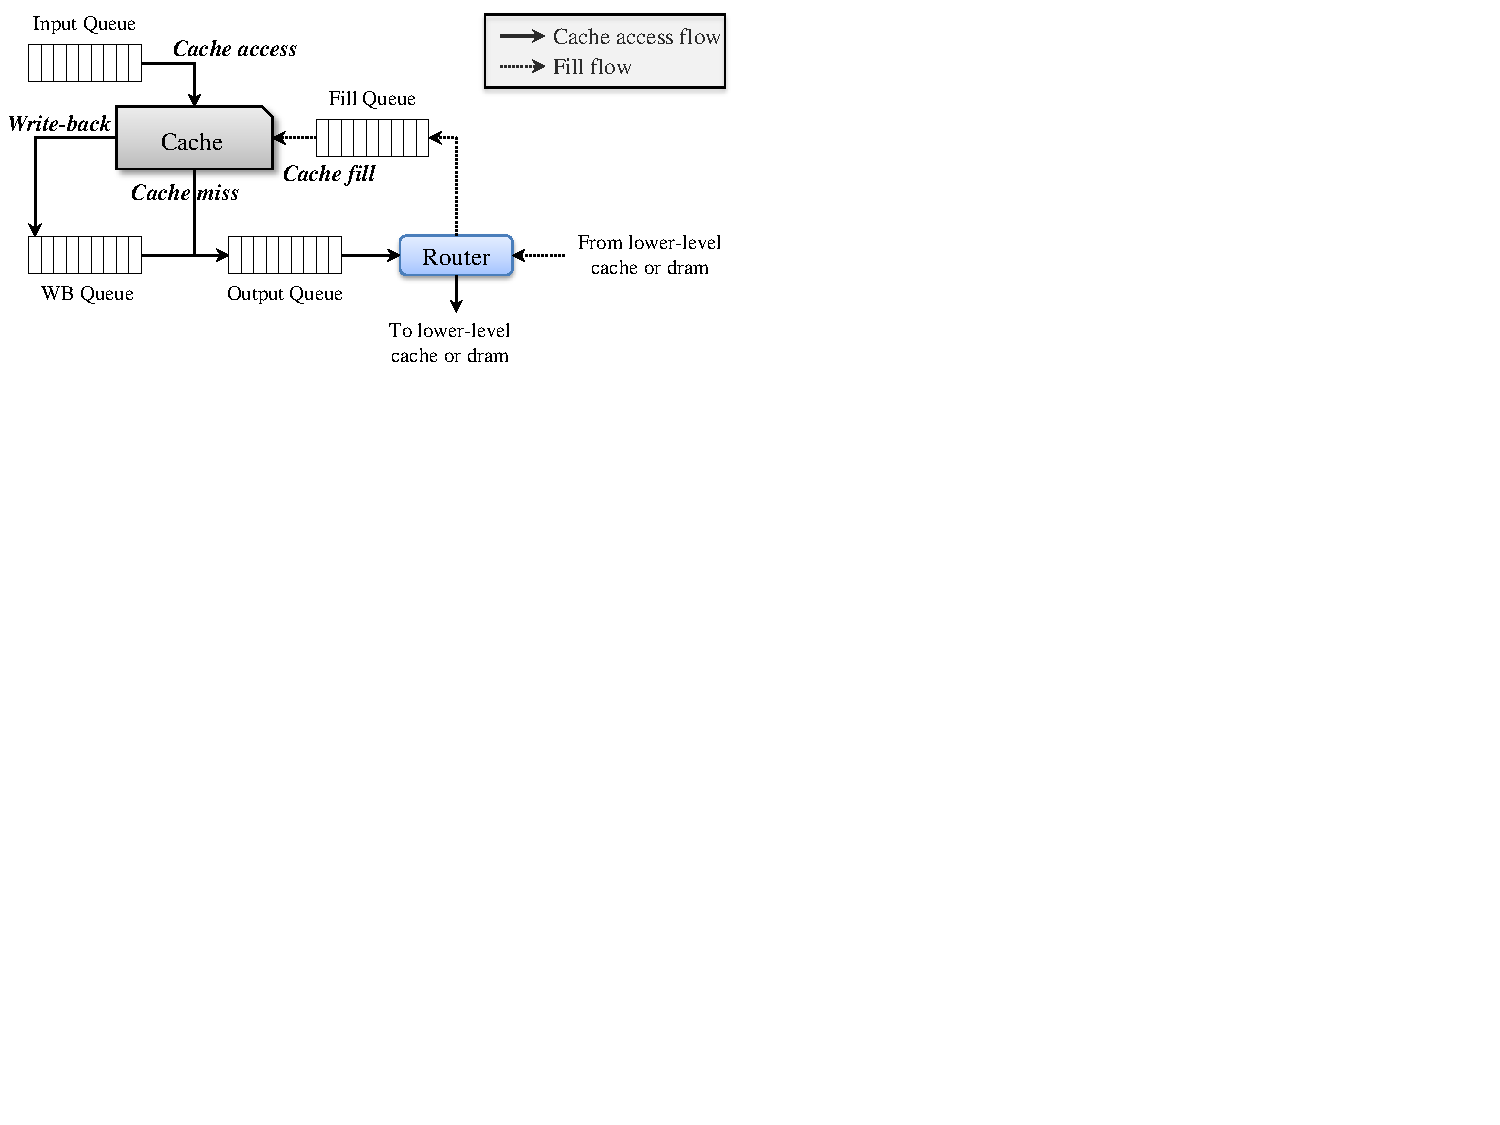
\includegraphics{figs/cache}
\caption{The cache structure.}
\label{fig:cache}
\end{figure*}


\subsection{The Queues}
\label{sec:queue}

All cache accesses flow from one queue to the other queue. 

\begin{itemize}
  \item input queue - to access a cache. Requests due to upper-level
  cache misses are inserted in this queue.

  \item output queue - as a result of a cache-miss, a request will be
  inserted into the output queue to be supplied data from the
  lower-level caches or DRAM.

  \item write-back queue - In \SIM, we model write-back caches. When a
  cache line is evicted and dirty, this line needs to be written back
  in the lower level. All write-back requests are initially inserted
  into the write-back queue.

  \item fill queue - requests in this queue tries to fill the data
  that is returned from the lower-level cache or DRAM.

  \item coherence queue - this queue is intended for handling
  coherence traffics, but this is currently not modeled.
\end{itemize}


\subsection{The Flows in the Cache Structure}
\label{sec:cache-flow}

\begin{itemize}

  \item Upper-level cache to input queue : upper-level cache miss

  \item input queue to cache : access the cache

  \item cache to output queue : cache miss and lower-level cache access

  \item cache to write-back queue : write-back requests

  \item write-back queue to output queue : to access lower-level cache

  \item output queue to the router : to access the lower-level cache
  through the on-chip interconnection network.

  \item router to the fill queue : the data from the lower-level cache
  or DRAM

\end{itemize}


\section{The Hierarchy}
\label{sec:memhierarchy}

\SIM maintains very flexible memory hierarchy. Each level of cache 
hierarchy is independent and \SIM defines the link between the
levels. Figure~\ref{fig:memory} shows the diagram of the memory
hierarchy in \SIM.

\begin{figure*}[htb]
\centering
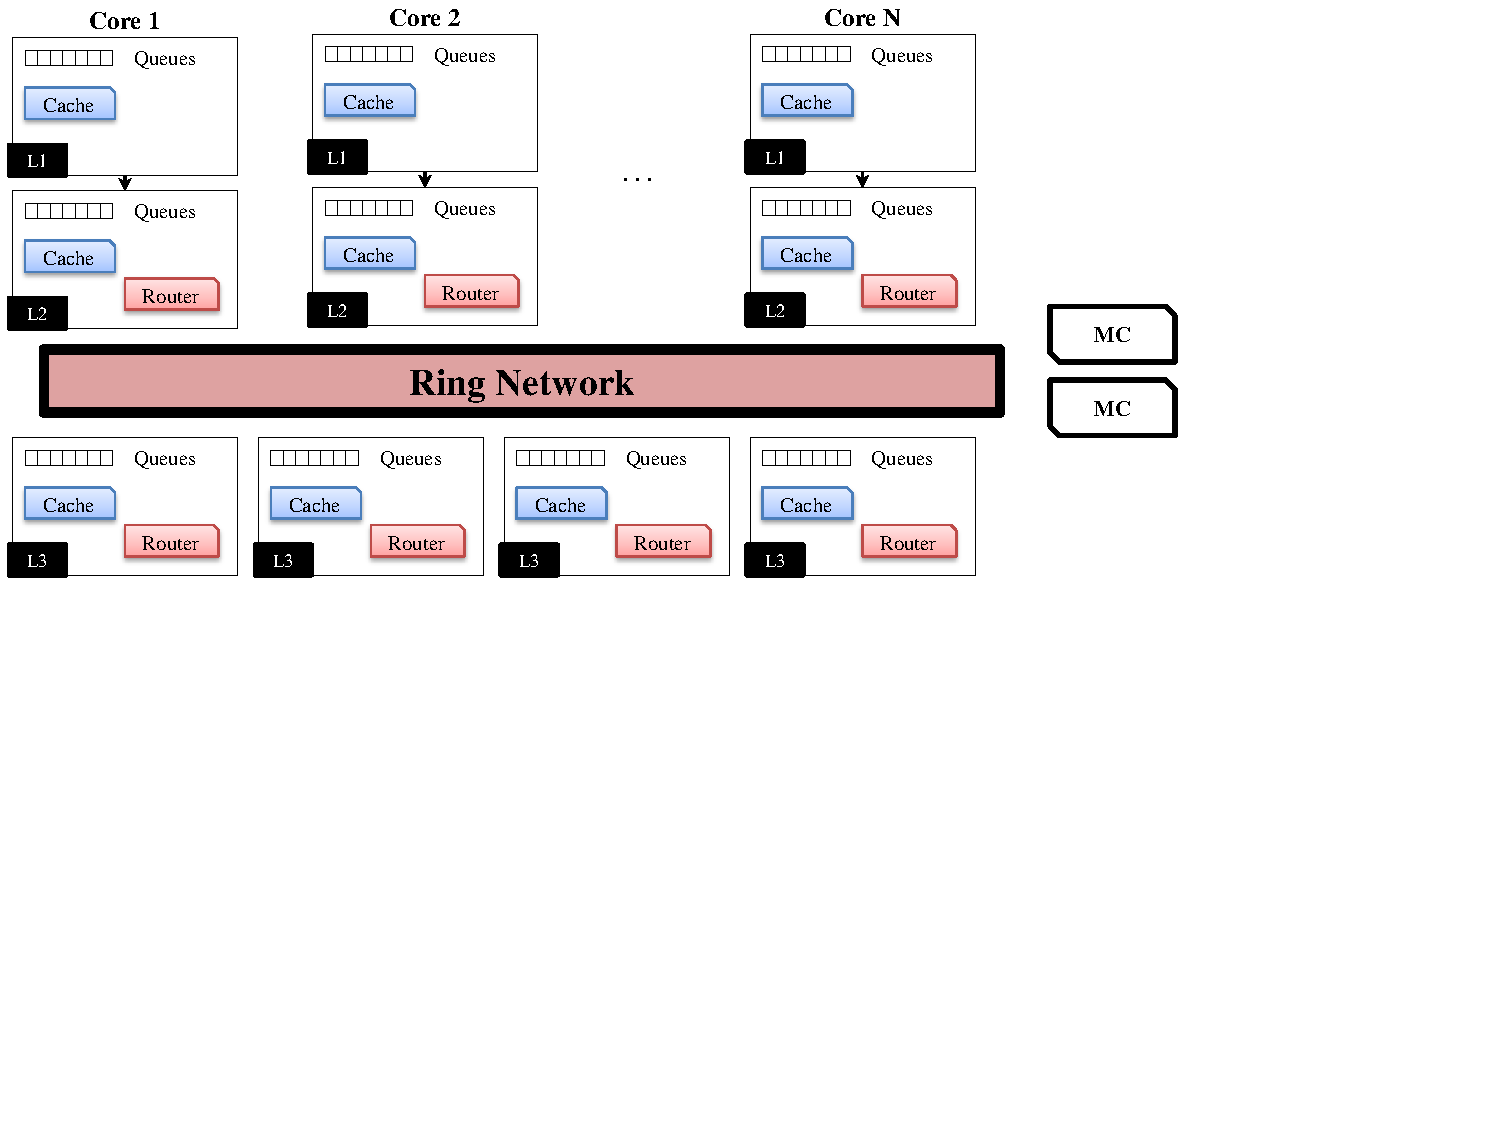
\includegraphics[width=6.5in]{figs/memory}
\caption{The memory system in \SIM.}
\label{fig:memory}
\end{figure*}



Here are some basics.


\begin{itemize}
  \item There are three levels (L1, L2, and L3) of caches in the \SIM
  although L2 cache might be disabled in some configurations.

  \item All these caches and memory controllers are connected via
  on-chip interconnection network (currently, the default topology is
  ring).

  \item L1 and L2 caches are always private to each processors.

  \item The local router within a cache structure is enabled when
  necessary.

  \item L3 cache is unified (shared by all cores), but tiled based on
  the static bank partition. In other words, address regions are
  statically partitioned and each tile is responsible for sub regions.

\end{itemize}


For example, Figure~\ref{fig:level2cache} shows the example of 2-level
caches. Even though there are 3-level caches, L2 cache is disabled and
only its router is used by the L1 cache to access the interconnection
network. Since there is no additional latency between L1 and L2, we
can flexibly configure 2-level caches.


\begin{figure*}[htb]
\centering
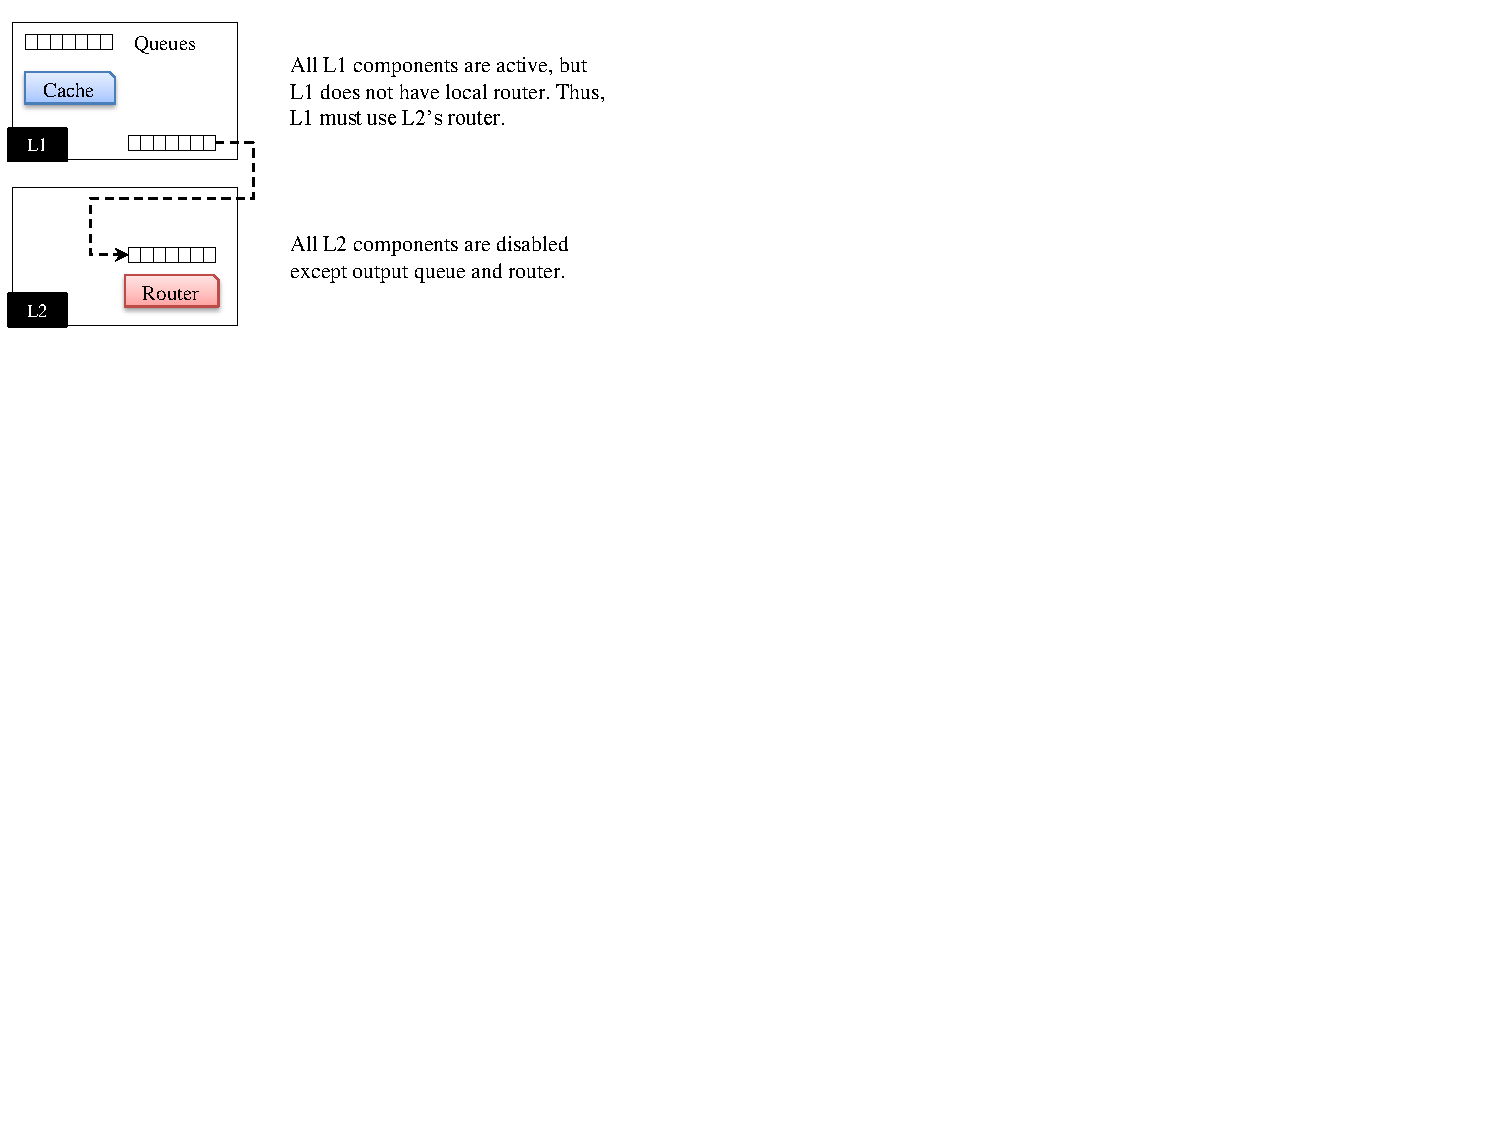
\includegraphics{figs/level2cache}
\caption{2-Level cache hierarchy.}
\label{fig:level2cache}
\end{figure*}


\section{How to Configure Cache Hierarchy} 

The cache hierarchy can be configured by setting 1) the link between
upper/lower level cache, 2) disability, and 3) router. The following
code is used in the \SIM cache initialization.

\begin{Verbatim}
void dcu_c::init(
  int next_id, // next level cache id
  int prev_id, // previous level cache id
  bool done, 
  bool coupled_up, // direct link with upper level cache
  bool coupled_down, // direct link with lower level cache
  bool disable, // disability
  bool has_router // router
);
\end{Verbatim}

\begin{description}
  \item[Router] When \textsf{has\_router} is set to \textit{false},
  the cache cannot directly access to the on-chip
  interconnection. Instead, it has to go through lower-level cache's
  interface. Therefore, \textsf{coupled\_down} must set
  to \textit{true} and appropriate \textsf{next\_id} must be set. In
  this way, the output queue of the cache is connected directly to the
  input queue of the next level (lower) cache.

  \item[Disability] When \textsf{disable} is set to \textit{true}, the
  cache is disabled. When a request is inserted from the upper level
  cache, it will be directly inserted into the output queue. This
  feature has been used for modeling 2-level cache hierarchy. As
  Figure~\ref{fig:level2cache} shown, L1 and L3 caches are active, but
  L2 cache is disabled. However, the L1 cache does not have a router,
  so it needs to use the router of the L2
  cache. Therefore, \textsf{has\_router} must be set to \textit{true}.

  \item[Link] As mentioned in the Section~\ref{sec:memhierarchy}, the
  L1 and L2 caches are always private to a processor. All L1 misses
  should go through the L2 cache without accessing the interconnection
  network. To this end, the direct link must be set between the L1 and
  L2 caches. Therefore, \textsf{coupled\_down} and \textsf{next\_id}
  must be set for the L1 cache and \textsf{coupled\_up}
  and \textsf{prev\_id} must be set for the L2 cache. Note that the
  link is always bi-directional.

\end{description}

\subsection{Example of Different Cache Hierarchy}

We provide several example of the cache hierarchy.

\begin{itemize}
\ignore{
  \item Intel Core~\cite{core2duo} microarchitecture has two-level of
  caches. The last-level cache might be tiled, but if the L2 cache
  tries to access the closest the L3 tile, it does not have to access
  through the interconnection. All communications will be made through
  the direct link. However, if the L2 cache accesses the remote L3
  tile, it goes through the interconnection. Note that the number of
  cores (L1 and L2 caches) and the number of the L3 tiles must be the
  same.

  \smallskip
  \begin{lstlisting}
  // class l2_coupled_local_c
  \end{lstlisting}
  \smallskip
}

  \item Intel Nehalem~\cite{nehalem} and Sandy
  Bridge~\cite{sandybridge} microarchitecture have three-level of
  caches. The last-level cache is tiled, but if the L2 cache tries to
  access the closest L3 tile, it does not have to access through the
  interconnection. All communications will be made through the direct
  link. However, if the L2 cache accesses the remote L3 tile, it goes
  through the interconnection. Note that the number of cores (L1 and
  L2 caches) and the number of the L3 tiles must be the same in this
  configuration.

  \smallskip
  \begin{lstlisting}
  // class l3_coupled_network_c
  for (int ii = 0; ii < m_num_core; ++ii) {
    // next_id, prev_id, done, coupled_up, coupled_down, disable, router
    m_l1_cache[ii]->init(ii, -1, false, false, TRUE, false, false);
    m_l2_cache[ii]->init(ii, ii, true,  TRUE,  TRUE, false, TRUE);
    m_l3_cache[ii]->init(-1, ii, false, TRUE,  false,false, TRUE);
  }

  \end{lstlisting}
  \smallskip

  \item NVIDIA G80~\cite{g80} architecture does not have
  hardware-managed caches. Thus, all three levels are connected each
  other and disabled. Only the L3 cache has a router to access DRAM.

  \smallskip
  \begin{lstlisting}
  // class no_cache_c
  for (int ii = 0; ii < m_num_core; ++ii) {
    // next_id, prev_id, done, coupled_up, coupled_down, disable, router
    m_l1_cache[ii]->init(ii, -1, false, false, TRUE,  TRUE, false);
    m_l2_cache[ii]->init(ii, ii, true,  TRUE,  TRUE,  TRUE, false);
    m_l3_cache[ii]->init(-1, ii, false, TRUE,  false, TRUE, TRUE);
  }

  \end{lstlisting}
  \smallskip

  \item NVIDIA Fermi~\cite{fermi} architecture has private L1 cache
  and unified L2 cache shared by all cores. The L1 and L2 caches are
  linked. The L2 cache has been disabled, but has a router
  enabled. The L3 is not linked with others, but it is enabled and has
  a router.

  \smallskip
  \begin{lstlisting}
  // class l2_decoupled_network_c
  // next_id, prev_id, done, coupled_up, coupled_down, disable, router
  for (int ii = 0; ii < m_num_core; ++ii) {
    m_l1_cache[ii]->init(ii, -1, false, false, TRUE,  false, false);
    m_l2_cache[ii]->init(-1, ii, true,  TRUE,  false, true,  true);
  }

  for (int ii = 0; ii < m_num_l3; ++ii) {
    // next_id, prev_id, done, coupled_up, coupled_down, disable, router
    m_l3_cache[ii]->init(-1, -1, false, false, false, false, true);
  }

  \end{lstlisting}
  \smallskip
  
  \item In general 2-D Topology (Mesh, Torus), we assume each core has
  private L1 and L2 caches, but access to the L3 cache must be
  communicated through the interconnection network. The L1 and L2
  caches are both enabled and linked, but only the L2 cache has a
  router. The L3 cache is not linked with others and the communication
  is made through the interconnection network.

  \smallskip
  \begin{lstlisting}
  // class l3_decoupled_network_c
  // next_id, prev_id, done, coupled_up, coupled_down, disable, router
  for (int ii = 0; ii < m_num_core; ++ii) {
    m_l1_cache[ii]->init(ii, -1, false, false, TRUE,  false, false);
    m_l2_cache[ii]->init(-1, ii, true,  TRUE,  false, false, TRUE);
  }

  for (int ii = 0; ii < m_num_l3; ++ii) {
    // next_id, prev_id, done, coupled_up, coupled_down, disable, router
    m_l3_cache[ii]->init(-1, -1, false, false, false, false, TRUE);
  }

  \end{lstlisting}
  \smallskip

\end{itemize}

\section{DRAM Module} 

\SIM also models detail memory controllers: timing constraint, 
bandwidth, and scheduling. Section~\ref{sec:param-dram} describes how
to configure DRAM parameters.

The DRAM controller consists of multiple banks with one ore more
channels. Each bank has own request buffer and bank scheduler picked

\begin{itemize}
  \item The bank scheduler picks a request based on the policy (FCFS,
  FRFCFS, ...) if nothing is served now.

  \item The channel scheduler picks a request from command-ready banks
  (usually oldest request first). Based on the command, appropriate
  timing constraint is enforced to the bank.

  \item Once the column access signal is sent, the data is prepared
  from the DRAM chip (load) or the data is sent to the DRAM chip
  (store). Among multiple data-ready banks, the channel scheduler
  picks a request based on the policy (oldest-first).

  \item When the data is ready/sent for a request, the data is
  supplied to the cache (load) or the request is completed (store).

  \item If there are memory requests with the same address, these
  requests are merged into one dram request. 

\end{itemize}



% LocalWords:  prev bool microarchitecture Nehalem num init NVIDIA FCFS FRFCFS


\clearpage
\section{The GPU Model}


We model our GPU cores similar to NVIDIA Fermi~\cite{fermi}.
%Figure~\ref{fig:g80} shows an overview of the GPU architecture that we modeled in our simulator. 
The GPU architecture consists of a scalable number of {\em streaming
multiprocessors} (SMs), each containing eight {\em streaming processor}
(SP) cores, two special function units (SFUs), a multithreaded
instruction fetch and issue unit, a read-only constant cache, and a
16KB read/write shared memory~\cite{lin:nic08}.
In our simulator SMs are names as cores and SPs are just one of the functional units. 


\ignore{
\begin{figure}[htb]
\centering
\psfig{file=figs/g80, angle=0, width=\figwidth}
\caption{An overview of the GPU architecture}
\label{fig:g80}
\end{figure}
}

The SM executes a batch of 32 threads together called a {\em
warp}. In the simulator, one warp is treated as one thread. 
The trace generator already formed a warp and stored them. 

\subsection{Changes to support GPU}
\subsubsection{Front-end changes}
The following components are modified to support GPUs. 
\begin{enumerate}
\item Handling divergent branch
\item Fetch scheduling (when to block a thread)
\end{enumerate}
\subsubsection{Scheduler}
Different scheduling policy can be implemented. The default is the round-robin policy. 

\subsubsection{Process Manager}

\begin{enumerate}
\item Block Dispatch: Threads are dispatched as a block granularity. 
The simulator waits until all threads within a block are finished 
before it dispatches another block. 
\item Occupancy: When a trace is generated from Ocelot, it also emits the number of required 
physical registers and memory usages. So the simulator uses that information to decide 
how many blocks can be allocated for each core. This value can be overwritten by a KNOB as well. 
\end{enumerate}

\subsubsection{Execution Stage}
Since one warp is treated as a functional unit, execution stage itself does not require too much change. Major changes are in handling uncoalesced memory  requests. 

\subsubsection{Memory system}
The simulator includes read-only cache, texture cache and constant cache to model GPUs. 

\ignore{



Executing a warp instruction applies the instruction to 32
threads, similar to executing a SIMD instruction like an SSE
instruction~\cite{sse} in X86. However, unlike SIMD instructions, the
concept of warp is not exposed to the programmers, rather programmers
write a program for one thread, and then specify the number of
parallel threads in a block, and the number of blocks in a kernel
grid. The Tesla architecture forms a warp using a batch of 32
threads~\cite{cuda:course, sc2008_cuda} and in the rest of the paper
we also use a warp as a batch of 32 threads.\ignore{\footnote{The CUDA
manual~\cite{cuda_manual} describes a half warp (16 threads) as a
minimum unit of execution. However, to simplify the model, we use only
warp as a minimum unit of execution.}}

All the threads in one block are executed on one SM together. One SM
can also have multiple concurrently running blocks. The number of
blocks that are running on one SM is determined by the resource
requirements of each block such as the number of registers and shared
memory usage. The blocks that are running on one SM at a given time
are called {\em active blocks} in this paper. Since one block
typically has several warps (the number of warps is the same as the
number of threads in a block divided by 32), the total number of
active warps per SM is equal to the number of warps per block times
the number of active blocks.

The shared memory is implemented within each SM multiprocessor as an
SRAM and the global memory is part of the offchip DRAM. The shared
memory has very low access latency (almost the same as that of
register) and high bandwidth. However, since a warp of 32 threads
access the shared memory together, when there is a bank conflict
within a warp, accessing the shared memory takes multiple cycles.

}


% LocalWords:  GPU NVIDIA SMs SFUs multithreaded SPs GPUs uncoalesced SIMD CUDA
% LocalWords:  SRAM offchip


\chapter{Overview of MacSim Code Structures}
\label{sec:codetop}


\section{sim}

\section{run\_a\_cycle}

\section{core}


\clearpage
\section{Process Manager/Thread Scheduler}

MacSim uses a common Process Manager/Thread Scheduler for both CPU threads and
GPU warps. For each application that is to be simulated, the Process Manager
creates a process and also creates the threads/warps in the application. Based
on the simulation configuration, the Process Manager assigns cores to each
application, these cores are dedicated to the application. In case of CPU
applications, only the main thread of the application is launched first. The
trace config that is input to the simulator specifies in terms of instructions
executed by the main thread when each child thread should be started. When a
child thread becomes ready for execution, the Process Manager is responsible
for assigning the child threads to cores. In case of GPU applications, the
Process Manager creates warps and forms thread blocks from these warps. The
thread blocks are assigned to cores according to the maximum number of blocks
supported by the core. Though the term core is commonly used for both X86 cores
and GPU cores, we want to clarify that a X86 thread can run only on a core
specified as X86 and a warp/block can run only a core specified as a GPU core.
Threads/warps once assigned to a core, remain attached to the core until they
terminate. When a thread or a warp terminates, the Process Manager is invoked
again for updating bookkeeping information. When it is determined that an
application can terminated, based on the simulation parameters, the Process
Manager could repeat the simulation of the application until the termination
condition is met.



Some of the key data structures used by the Process Manager are:

\begin{description}

\item [process\_s] For each application that is to be simulated, the process manager
creates a instance of type process\_s. This structure includes information such
as process id, start information of threads, number of threads (warps) in
application, number of threads (warps) created, number of threads (warps)
  terminated, list of cores on which the application can run and so on.

\item [thread\_s] This structure is analogous to the task struct maintained by an
operating system kernel. Each CPU thread and GPU warp has an instance of
thread\_s structure. This structure includes fields for thread id, block id,
  pointer to trace file, process to which the thread belongs and other fields. 

\item [block\_schedule\_info\_s] Bookkeeping structure representing thread blocks in
a GPGPU application. This structure contains fields for number of warps in a
block, number of terminated warps, core to which the block is assigned and so
on.

\item [thread\_trace\_info\_node\_s] Wrapper structure around thread\_s used by
Process manager to track threads/warps yet to be assigned cores.

\end{description}


%%%%%%%%%%%%%%%%%%%%%%%%%%%%%%%%%%%%%%%%%%%%%%%%%%%%%%%%%%%%%%%%%%%%%%%%
\chapter{Adding to \SIM}
\label{sec:add_macsim}
%%%%%%%%%%%%%%%%%%%%%%%%%%%%%%%%%%%%%%%%%%%%%%%%%%%%%%%%%%%%%%%%%%%%%%%%
In this chapter procedure to add new policies, predictors and prefetcher 
to \SIM are explained.

%%%%%%%%%%%%%%%%%%%%%%%%%%%%%%%%%%%%%%%%%%%%%%%%%%%%%%%%%%%%%%%%%%%%%%%%
\section{New DRAM Policy}
%%%%%%%%%%%%%%%%%%%%%%%%%%%%%%%%%%%%%%%%%%%%%%%%%%%%%%%%%%%%%%%%%%%%%%%%


To implement a new DRAM scheduling policy, a class that extends
\textit{dram\_controller\_c} has to be defined. This class should
overload the \textit{schedule()} function which should return the next
DRAM request to be serviced according to the policy. Please refer to
class \textit{dc\_frfcfs\_s} defined in dram.cc/h for a sample. In
addition to the class, define a wrapper function that returns an
instance of the class (see \textit{dram.cc} for an example) and
register the class with the DRAM factory (see \textit{see
register\_functions() in \textit{macsim.cc}}.


%%%%%%%%%%%%%%%%%%%%%%%%%%%%%%%%%%%%%%%%%%%%%%%%%%%%%%%%%%%%%%%%%%%%%%%%
\section{New Instruction Scheduler}
%%%%%%%%%%%%%%%%%%%%%%%%%%%%%%%%%%%%%%%%%%%%%%%%%%%%%%%%%%%%%%%%%%%%%%%%

Define a class that extends \textit{schedule\_c} and overloads at least the
\textit{run\_a\_cycle()} function. Other functions may be overloaded to
maintain a consistent code structure across the different instruction
schedulers. After defining the new scheduler, add code to \textit{core.cc} to
instantiate the new scheduler instead of one of the provided schedulers.

%%%%%%%%%%%%%%%%%%%%%%%%%%%%%%%%%%%%%%%%%%%%%%%%%%%%%%%%%%%%%%%%%%%%%%%%
\section{New policy for assigning thread blocks to GPU cores}
%%%%%%%%%%%%%%%%%%%%%%%%%%%%%%%%%%%%%%%%%%%%%%%%%%%%%%%%%%%%%%%%%%%%%%%%

In \textit{process\_manager\_c::sim\_schedule\_thread\_block()} add (or modify)
code to determine the id of the block that will be assigned to the core based
on the new policy. The list of ready blocks can be obtained via
\textit{m\_block\_schedule\_info} member of the \textit{macsim\_c} object that
is created for the simulation.

%%%%%%%%%%%%%%%%%%%%%%%%%%%%%%%%%%%%%%%%%%%%%%%%%%%%%%%%%%%%%%%%%%%%%%%%
\section{New Fetch Policy}
\label{sec:modify:fetch}
%%%%%%%%%%%%%%%%%%%%%%%%%%%%%%%%%%%%%%%%%%%%%%%%%%%%%%%%%%%%%%%%%%%%%%%

There are several steps to add a new thread fetching policy. We will
provide an example with round-robin fetch policy, which is already
provided by \SIM.

\begin{enumerate}[Step 1.]
\item Define a new fetch policy in \Verb+class frontend_c+.
\begin{Verbatim}
// frontend.h
class frontend_c {
  ...
  int fetch_rr(void);
  ...
}
\end{Verbatim}

\item Implement this new policy.

\item Register this new policy in \Verb+macsim.cc+.
\begin{Verbatim}
fetch_factory_c::get()->register_class("rr", fetch_factory);
\end{Verbatim}


\item Assign this policy to \Verb+MT_fetch_Scheduler+ in \Verb+frontend.cc+.
\begin{Verbatim}
if (policy == ``rr'') {
  MT_fetch_scheduler = &frontend_c::fetch_rr;
}
\end{Verbatim}

\item Enable this new branch predictor by setting \Verb+KNOB_FETCH_POLICY+.
\begin{Verbatim}
./macsim --fetch_policy=rr     -- in the commandline
fetch_policy rr                -- in the params.in
\end{Verbatim}
\end{enumerate}


%%%%%%%%%%%%%%%%%%%%%%%%%%%%%%%%%%%%%%%%%%%%%%%%%%%%%%%%%%%%%%%%%%%%%%%%
\section{New Branch Predictor}
%%%%%%%%%%%%%%%%%%%%%%%%%%%%%%%%%%%%%%%%%%%%%%%%%%%%%%%%%%%%%%%%%%%%%%%%

There are several steps to add a new branch predictor. We will provide
an example with gshare~\cite{mcf93} branch predictor, which is already
provided by \SIM.

\begin{enumerate}[Step 1.]
  \item Define a new class which inherits \Verb+class bp_dir_base_c+
\begin{Verbatim}
class bp_gshare_c : public bp_dir_base_c {};
\end{Verbatim}

  \item Define and implement other necessary features of a new branch
    predictor. Especially, override \Verb+pred()+, \Verb+update()+,
    and \Verb+recover()+ functions.
\begin{Verbatim}
uns8 bp_gshare_c::pred(uop_c* uop) {...}
void bp_gshare_c::update(uop_c* uop) {...}

\end{Verbatim}

  \item Add a policy to the branch predictor factory in
    \Verb+macsim.cc+ and to the allocator in \Verb+bp.cc+.

\begin{Verbatim}
// macsim.cc macsim_c::register_functions()
bp_factory_c::get()->register_class(``gshare'', default_bp);

// bp.cc
bp_dir_base_c* default_bp(macsim_c* simBase)
{
  ...
  else if (bp_type == ''gshare'')
    new_bp = new bp_gshare_c(simBase);
  ...
}
\end{Verbatim}

  \item Enable this new branch predictor by setting \Verb+KNOB_BP_DIR_MECH+.
\begin{Verbatim}
./macsim --bp_dir_mech=gshare     -- in the commandline
bp_dir_mech gshare                -- in the params.in
\end{Verbatim}
\end{enumerate}


%%%%%%%%%%%%%%%%%%%%%%%%%%%%%%%%%%%%%%%%%%%%%%%%%%%%%%%%%%%%%%%%%%%%%%%%
\section{New Hardware Prefetcher}
%%%%%%%%%%%%%%%%%%%%%%%%%%%%%%%%%%%%%%%%%%%%%%%%%%%%%%%%%%%%%%%%%%%%%%%%

There are several steps to add a new hardware prefetcher. We will provide
an example with a stride~\cite{iac:spr04} prefetcher, which is already
provided by \SIM.

\begin{enumerate}[Step 1.]
  \item Define a new class which inherits \Verb+class pref_base_c+
\begin{Verbatim}
class pref_stride_c : public pref_base_c {};
\end{Verbatim}

  \item Define and implement other necessary features of a new
    hardware prefetcher. Especially, override several function.
\begin{Verbatim}
void init_func(int);                            // on initiation of prefetch request
void done_func();                               // when a prefetch request is installed
void l1_miss_func(int, Addr, Addr, uop_c*);     // on L1 miss
void l1_hit_func(int, Addr, Addr, uop_c*);      // on L1 hit
void l1_pref_hit_func(int, Addr, Addr, uop_c*); // on L1 prefetch hit
void l2_miss_func(int, Addr, Addr, uop_c*);     // on L2 miss
void l2_hit_func(int, Addr, Addr, uop_c*);      // on L2 hit
void l2_pref_hit_func(nt, Addr, Addr, uop_c*);  // on L2 prefetch hit
\end{Verbatim}

  \item Add a prefetcher to the prefetcher factory in \Verb+pref_factory.cc+.

\begin{Verbatim}
// pref_factory.cc
void pref_factory(...)
{
  pref_base_c* pref_stride = new pref_stride_c(...);
  pref_table.push_back(pref_stride);
  ...
}
\end{Verbatim}

  \item Enable this new hardware prefetcher by setting
    \Verb+KNOB_PREF_STRIDE_ON+ (please refer to pref\_stride.cc
    pref\_stride\_c::pref\_stride\_c()). \textit{Note that the way we
      simulate hardware prefetchers are not same as other modules.}
\begin{Verbatim}
switch (type) {
  case UNIT_SMALL:
    knob_enable = *m_simBase->m_knobs->KNOB_PREF_STRIDE_ON;
      break;
    case UNIT_MEDIUM:
      knob_enable = *m_simBase->m_knobs->KNOB_PREF_STRIDE_ON_MEDIUM_CORE;
      break;
    case UNIT_LARGE:
      knob_enable = *m_simBase->m_knobs->KNOB_PREF_STRIDE_ON_LARGE_CORE;
      break;
}

./macsim --pref_stride_on[,medium_core, large_core]=1
pref_stride_on[,medium_core, large_core] 1
\end{Verbatim}
\end{enumerate}



\chapter{Debugging}
\label{sec:debugging}
TBD 
\section{Forward Progress Error}
TBD 



\section{Debugging with Debugging Messages}

To check the correctness of the module, We provide debugging features
with text-based debugging messages. For example,

\begin{Verbatim}
debug message example
\end{Verbatim}

You can define anywhere. Opt version will nullify these statement for
performance purpose.

enable variable

To enable debug messages \Verb+make dbg+ and 

\begin{Verbatim}
debug_cycle_start
debug_cycle_end
\end{Verbatim}

debug macros are defined in \Verb+macsim-top/trunk/def/src/debug_macros.h+

debug macro is very similar to \Verb+printf+ function.

\begin{Verbatim}
_debug(debug_variable, const char * format, ... )
\end{Verbatim}

\begin{Verbatim}
#define DEBUG(args...) _DEBUG(*m_simBase->m_knobs->KNOB_DEBUG_MEM, ## args)
\end{Verbatim}


useful data for 

\begin{Verbatim}
core id
thread id
uop num
inst num
vaddr
req_id
\end{Verbatim}


To add a new debug stage, you need to add a debug knob variable in debug.param.def


%\begin{Verbatim}
%DEBUG(
%\end{Verbatim}

%the meanting of debug statements. 
%How to turn on debug flags for different modules

%\subsection{DE


%\subsection{Debug Knob Variables}

%All debug variabls are defined in \Verb+macsim-top/trunk/def/debug.param.def+



%how to enable

%debug_start_cycle debug_end_cycle

%grep core_id thread_id

%how to add a new stage


%\subsection{How to Add Debugging Messages}

%\begin{enumerate}
%\item Add a new debug variable
%\item Add debug macro in files
%\item DEBUG


\chapter{Internal Users Only Manual}
\section{Regression Tests}
\label{sec:regression}

Let's say your current working directory name is macsim-working

\begin{enumerate}

\item Step 1: you need to get a clean copy of macsim again. let's say you are getting a new copy in macsim-regression directory.

{\texttt svn co https://svn.research.cc.gatech.edu/macsim/trunk macsim-regression --username user }

\item Step 2: you have to get a simulator tool, which is still in the hparch svn repository.

\item Step 3: go to macsim-regression/trunk/bin directory and execute regression\_gen.py which is in your tool directory.

\item Step 4: go to macsim-working/trunk/bin directory and execute regression\_test.py which is in your tool directory. 

\end{enumerate}


\section{How to Add New Files in MacSim}

\begin{Verbatim} 
run 'patch -p0 -i macsim-internal.patch', this will update <macsim_root>/.obj/Makefile.am to include the internal files in the build 
\end{Verbatim}


\section{What to use internal directory}

TBD




\chapter{FAQ}
\label{sec:faq}

\begin{enumerate}
\item I'd like to add a new file in Macsim. What should I do? 

\begin{verbatim}  run 'patch -p0 -i macsim-internal.patch', this will update <macsim_root>/.obj/Makefile.am to include the internal files in the build 
\end{verbatim}
\end{enumerate}

%
\clearpage
\section{Tools}
\label{sec:tool}
TBD 
\subsection{Trace Reader}
TBD 

%
\clearpage
\section*{Acknowledgments}

Acknowledgments...





\bibliographystyle{ieee}
\bibliography{ref}


%\begin{thebibliography}{9}
%\bibliography{ref}
%\end{thebibliography}



\clearpage
\appendix

\chapter{Coding Style Guideline}


\section{Naming Conventions}

Names should be as descriptive as possible, do not hesitate to use
long names.  Shorten names only when the purpose of the name can still
be understood clearly.


\subsection{Classes}

\begin{itemize}

  \item \textbf{Class names} should use lower case alphabets only.  If the name
consists of multiple words, then the words should be separated using
the underscore character. Class names should end with c.  Eg.

\begin{Verbatim}
class  my_class_c;
\end{Verbatim}


  \item \textbf{Class member variables} should use the prefix m .  Member variable
names should use lower case alphabets only, multiple words should be
separated using the underscore character.  Eg.

\begin{Verbatim}
int  m_instance_variable;
\end{Verbatim}


  \item \textbf{Accessor i.e, get/set, member functions} should use
the names of the corresponding member variables without the m
suffix. In addition, the set functions should use the prefix set ,
while no prefix is needed for the get functions.  Eg.


\begin{Verbatim}
int  m_my_variable;
...
...
void  set_my_variable(int);
int  my_variable();
\end{Verbatim}


  \item \textbf{Other member functions} should always start with a
verb, multiple words should be separated with the underscore character
and no upper case letters are allowed.  Eg.

\begin{Verbatim}
int  access_cache();
\end{Verbatim}


  \item Example class declaration

\begin{Verbatim}
class  my_class_c  {
  private:
    int  m_var_one;
    bool  m_var_two;
    ...
    ...

    void  set_var_one(int);
    int  var_one();
    ...
    int  check_values();
};
\end{Verbatim}

\end{itemize}





\subsection{Structures}

\begin{itemize}

  \item Structure names should use lower case alphabets only. If the
name consists of multiple words, then the words should be separated
using the underscore character. Structure names should end with s. Eg.

\begin{Verbatim}
struct  my_struct_s;
\end{Verbatim}

  \item Do not use any prefix or suffix for structure member
  variables.

  \item Example structure declaration

\begin{Verbatim}
typedef struct my_type_s  {
  type field_one;
  type field_two;
}  my_type_s;
\end{Verbatim}

\end{itemize}





\subsection{Other Types}

Other user defined types should use only lower case letters with
multiple words being separated by the underscore character. These
types should use the suffix t.  Eg.

\begin{Verbatim}
typedef  std::map<int,  std::list<int>  > my_type_t;
\end{Verbatim}


\subsection{Global Variables}

Global variable names should use the prefix g and use lower case
letters only, multiple words should be separated by the underscore
character.  Eg.

\begin{Verbatim}
int  g_my_global_variable;
\end{Verbatim}


\subsection{Local Variables}

Local variables follow the same convention as global variables, except
that they do not require the g prefix.  Eg.

\begin{Verbatim}
int  my_local_variable;
\end{Verbatim}


\subsection{Constant  Variables}

Constant variables follow the same convention as global variables,
except that they use the prefix k , instead of g .  Eg.

\begin{Verbatim}
const  int  k_my_const  = 25;
\end{Verbatim}


\subsection{Macros}

Macro names should use upper case letters only with multiple words
being separated my underscores. Eg.

\begin{Verbatim}
#define  MAX_NUM_THREADS  8192
\end{Verbatim}




\section{Formatting and Readability}

\subsection{Indentation}

Use only spaces for indentation, do not use tabs.  The indentation
must be two spaces wide.


\subsection{Variable Declaration}

Variables should be declared at the point in the code where they are
needed, and should be assigned an initial value at the time of
declaration.


\subsection{Control Statements and Function Definitions}

\begin{itemize}

  \item For \textit{if}, \textit{for}, \textit{while}
and \textit{switch} statements, there should be a single single space
between the keyword and the opening parenthesis.  The opening curly
brace should appear on the same line as the statement and there should
be a single space between the closing parenthesis and the opening
curly brace.  The opening curly brace following a do statement must
also follow the same rules.  The \textit{while} of a \textit{do while}
loop should be on the same line as the closing parenthesis of the loop
body and should be separated from the closing parenthesis by a single
space.  Eg.

\begin{Verbatim}
//correct
if (condition)  { 
  statement 1; 
  statement 2;
}

//correct
for  (int  ii = 0;  ii < N;  ++ii)  {
  statement 1;
  statement 2;
}

//correct
while  (condition)  { 
  statement 1; 
  statement 2;
}

//correct
switch  (variable)  {
  condition 1: 
    statement 1; 
    break;
  condition 2: 
    statement 2; 
    break;
  default: 
    statement 3; 
    break;
}

//correct 
do {
  statement 1;
  statement 2;
} while (condition);
\end{Verbatim}



  \item \textit{else} statements should be on the line following the
closing parenthesis of the corresponding if block. There should be a
single space between the else keyword and the opening curly brace of
the else block. The same rules apply for \textit{else if} statements
as well.  Eg.

\begin{Verbatim}
//correct
if (test_cond)  {
...
}
else  {
...

}

//correct
if (test_cond)  {
...
}
else  if (another_cond)  {
...
}
\end{Verbatim}

  \item When defining functions, there should be no spaces between the
function name and the opening parenthesis, there should be a single
space between the closing parenthesis and the opening curly brace which
should appear on the same line as the function name.  Eg.

\begin{Verbatim}
//correct
int  my_func_defn(int  arg_a,  int  arg_b)  {
  ...
}
\end{Verbatim}
\end{itemize}


\subsection{Horizontal Spacing}

Except for when using the operators listed below use a single space
between the operator and the operands (note the slight difference in
using the comma operator).  For the operands listed below, spaces
should not be used.  List of operators which do not need horizontal
spacing:

\begin{Verbatim}
() [] ->    ++ -- + - ! ~  (type)  *  &   sizeof
\end{Verbatim}

Eg.

\begin{Verbatim}
i = j + k * i;     // correct 
i = j+k*i;         // wrong

array[i]  = j;     // correct 
array [i] = j;     // wrong

my_func(a, b, c);  // correct 
my_func(a,b,c);    // wrong
\end{Verbatim}



\subsection{Statements}

Each statement should be on its own line, this applies to variable
declarations as well. Eg.

\begin{Verbatim}
int i = 0;          // correct 
int j = 0;          // correct
int i = 0,  j = 0;  // wrong 
i++;                // correct
j++;                // correct

i++;  j++;          // wrong 
i = 0;  j = 0;      // Wrong
\end{Verbatim}



\subsection{Column Length}

Lines should not exceed more than 80 characters in length.  If a line
is longer than 80 characters, split it into multiple lines.


\section{Header Files and Include Directives}

\begin{itemize}

  \item All header files should have an ``include guard'' to prevent
  accidental inclusion of the file multiple times in a single
  compilation unit.  The include guard should be named after the file
  name.  Eg.

\begin{Verbatim}
// in  pref_common.h
#ifndef  PREF_COMMON_H  #define  PREF_COMMON_H
...
...
#endif
\end{Verbatim}


  \item Avoid including header files in other header files by using
  forward declaration.

  \item All include directives should be grouped with system files
  listed first, followed by normal simulator header files.
\end{itemize}

\section{Comments}

Use Doxygen style comments. More to be added.


\section{Other Rules}

\begin{itemize}

  \item Avoid C style coding, try to build and use classes as much as
    possible.

  \item Define types which will not have functions other that accessor
    functions (and constructor and destructor) as structures. Use
    classes only if functions other than set/get will be needed.

  \item Definition of constructors and destructors (for both classes
    and structs) and class member functions should not be included in
    header files, unless the definitions are very small.

  \item Declare all global variables in global vars.h and define them
    in main.cc.

  \item More to be added.
\end{itemize}




% LocalWords:  Eg Accessor bool struct typedef const NUM cond func defn arg
% LocalWords:  sizeof ifndef endif Doxygen accessor destructors structs


\end{document}

%\bibliographystyle{ieee}
%\bibliography{ref}


%%% Local Variables: 
%%% mode: latex
%%% TeX-master: t
%%% End: 
